% !TeX program = xelatex

\documentclass[
    aspectratio=169,
]{beamer}

\usepackage[table]{xcolor}
\usepackage{minted}
\usepackage{diagbox}
\usepackage{makecell}

\usetheme{gray-scott}

\AtBeginSection{
    \begin{frame}{Outline}
        \begin{columns}
            \begin{column}{0.5\linewidth}
                \tableofcontents[currentsection, sections=1-7]
            \end{column}
            \begin{column}{0.5\linewidth}
                \tableofcontents[currentsection, sections=8-16]
            \end{column}
        \end{columns}
    \end{frame}
}

\setminted{
    autogobble,
    fontsize=\small,
    xleftmargin=0.5em,
    xrightmargin=0.5em,
    breaklines,
    style=nord,
    bgcolor=black,
    formatcom=\color{white},
}

\setminted[text]{
    fontsize=\scriptsize,
}

% Captions
\renewcommand{\caption}[1]{%
    \begin{center}
        \color{darkgray}
        \scriptsize #1
    \end{center}%
}

\graphicspath{{images/}}

%Information to be included in the title page:
\title{Kokkos on GPU}
\subtitle{Gray-Scott School 2026}
\author{Mathieu Lobet, Paul Zehner, Paul Gannay, Hariprasad Kannan, Thomas Padioleau, Trévis Morvany}
\institute{CEA}
\date{2026-07-02}
\closing{
    \begin{description}[\hspace{0.355\linewidth}]
        \item[Kokkos website] \href{https://kokkos.org}{\texttt{kokkos.org}}
        \item[Kokkos repository] \href{https://github.com/kokkos}{\texttt{github.com/kokkos}}
        \item[Gray-Scott Kokkos repository] \href{https://github.com/Maison-de-la-Simulation/gray-scott-kokkos}{\texttt{github.com/Maison-de-la-Simulation/} \texttt{gray-scott-kokkos}}
    \end{description}%
}

\begin{document}

\begin{frame}[plain]
    \titlepage
\end{frame}

\begin{frame}{About this course}
    \begin{enumerate}
        \item CPU course (July the 25\textsuperscript{th})
        \item GPU course (today!)
    \end{enumerate}
\end{frame}

\begin{frame}[fragile]{Previously in Kokkos}
    \vspace{-1em}

    \begin{columns}
        \begin{column}{0.5\linewidth}
            \begin{minted}[fontsize=\scriptsize]{C++}
                #include <Kokkos_Core.hpp>

                int main(int argc, char* argv[]) {
                    Kokkos::ScopeGuard kokkos(argc, argv);

                    Kokkos::View<int **>
                        view("view", 10, 20);

                    Kokkos::parallel_for(
                        "compute",
                        Kokkos::MDRangePolicy<
                            Kokkos::Range<2>
                        >({0, 0}, {10, 20}),
                        KOKKOS_LAMBDA (int i, int j) {
                            view(i, j) = i + j;
                        }
                    );
                }
            \end{minted}
        \end{column}
        \begin{column}{0.5\linewidth}
            \small
            \begin{itemize}
                \item \mintinline{C++}|#include <Kokkos_Core.hpp>| the main Kokkos header
                \item \mintinline{C++}|ScopeGuard| or \mintinline{C++}|initialize|/\break\mintinline{C++}|finalize| before or around Kokkos code
                \item \mintinline{C++}|View| for multidimensional containers
                \item \mintinline{C++}|parallel_for| for parallel loops
                \item \mintinline{C++}|parallel_reduce| for parallel reductions
                \item \mintinline{C++}|RangePolicy| for single-dimension iteration spaces
                \item \mintinline{C++}|MDRangePolicy| for multidimensional iteration spaces
                \item \mintinline{C++}|KOKKOS_LAMBDA| for the lambdas
            \end{itemize}
        \end{column}
    \end{columns}
\end{frame}

\begin{frame}{Outline}
    \begin{columns}
        \begin{column}{0.5\linewidth}
            \tableofcontents[sections=1-7]
        \end{column}
        \begin{column}{0.5\linewidth}
            \tableofcontents[sections=8-16]
        \end{column}
    \end{columns}
\end{frame}

\section{Moving to a GPU backend}

\begin{exerciseframe}{Initialization}
    \begin{columns}
        \begin{column}{0.65\linewidth}
            \begin{minted}[breakafter={/},fontsize=\scriptsize]{sh}
                REPO=docker://gitlab-registry.in2p3.fr/thomas.padioleau/gray-scott-kokkos

                # pick one
                IMAGE=kokkos_gpu_interactive
                IMAGE=kokkos_gpu_interactive_jupyter
                IMAGE=kokkos_gpu_interactive_vscode
                IMAGE=kokkos_gpu_learning_platform_code_server

                apptainer pull $REPO/$IMAGE:latest

                srun ... --pty /bin/bash

                apptainer run --nv ${IMAGE}_latest.sif

                # if you didn't attend last week session
                cp -r /home/jovyan/Examples $HOME/gray_scott_kokkos

                cd $HOME/gray_scott_kokkos/exercises
            \end{minted}
        \end{column}
        \begin{column}{0.35\linewidth}
            \begin{itemize}
                \item Reserve a job for the day/half a day (ask your satellite staff)
                \item Run Apptainer with the downloaded SIF image
                \item \structure{If you didn't follow last week session,} duplicate the exercises in your home directory
            \end{itemize}
        \end{column}
    \end{columns}
\end{exerciseframe}

\begin{frame}{The notion of backend in Kokkos}
    \begin{itemize}
        \item Kokkos is compiled to target a specific backend
        \item Kokkos is portable until you compile it
        \item You need one compilation per backend
    \end{itemize}
    \begin{center}
        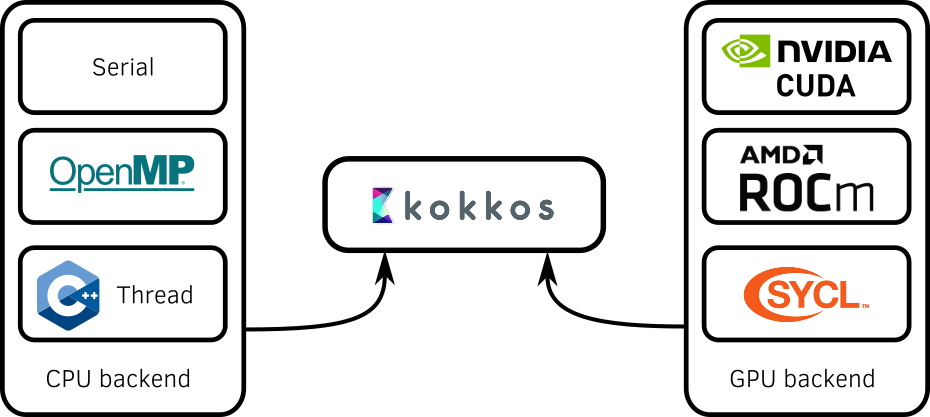
\includegraphics[width=0.6\textwidth]{kokkos_backend.png}
    \end{center}
\end{frame}

\begin{frame}[fragile]{Compiling Kokkos for a specific backend}
    \begin{columns}
        \begin{column}{0.45\linewidth}
            \begin{itemize}
                \item Add the option \texttt{-DKokkos\_ENABLE\_<BACKEND>=ON} to enable a specific backend
                \item Only one CPU backend and one GPU backend maximum can be compiled at a time (plus Serial backend)
            \end{itemize}
            \begin{minted}{bash}
                cmake \
                    -B ${build_dir} \
                    -DCMAKE_CXX_COMPILER=g++ \
                    -DKokkos_ENABLE_CUDA=ON \
                    ${other_options}
            \end{minted}
        \end{column}
        \pause
        \begin{column}{0.55\linewidth}
            \begin{center}
                \begin{table}{GPU backends}{ll}
                    Backend & Option \\\hline
                    Serial & \texttt{-DKokkos\_ENABLE\_SERIAL=ON} \\
                    OpenMP & \texttt{-DKokkos\_ENABLE\_OPENMP=ON} \\
                    Threads & \texttt{-DKokkos\_ENABLE\_THREADS=ON} \\
                    Cuda & \texttt{-DKokkos\_ENABLE\_CUDA=ON} \\
                    HIP & \texttt{-DKokkos\_ENABLE\_HIP=ON} \\
                    SYCL & \texttt{-DKokkos\_ENABLE\_SYCL=ON}
                \end{table}
            \end{center}
        \end{column}
    \end{columns}
\end{frame}

\begin{frame}{Compilers minimum version}
    \begin{center}
        \small
        \begin{table}{Compilers}{lll}
            Name       & Cmd.             & Min.\ ver. \\\hline
            Clang      & \texttt{clang++} & 15.0.0     \\
            GCC        & \texttt{g++}     & 10.4.0     \\
            Intel LLVM & \texttt{icpx}    & 2024.2.1   \\
            NVHPC      & \texttt{nvc++}   & 22.3       \\
            ROCM       & \texttt{hipcc}   & 6.2.0
        \end{table}
    \end{center}
\end{frame}

\begin{frame}{Warning regarding the backends}
    \begin{itemize}
        \item All backends \structure{may not have the same level of maturity}
        \item The backend environment (for instance Cuda) must be available on the target machine, \structure{Kokkos does not install it for you}!
    \end{itemize}
\end{frame}

\begin{frame}{Compiling Kokkos for a specific GPU architecture}
    \begin{columns}
        \begin{column}{0.37\linewidth}
            \begin{itemize}
                \item Add the architecture option \texttt{-DKokkos\_ARCH\_<NAME>=ON}
                \item CPU architecture is optional, for optimization
                \item GPU architecture is mandatory, deduced if device is present
                \item All CMake options are available \href{https://kokkos.org/kokkos-core-wiki/get-started/configuration-guide.html}{in the doc}
            \end{itemize}
        \end{column}
        \pause
        \begin{column}{0.63\linewidth}
            \begin{center}
                \small
                \begin{table}{GPU architectures}{ll}
                    GPU model & Option \\\hline
                    AMD MI300A & \texttt{-DKokkos\_ARCH\_AMD\_GFX942\_APU=ON} \\
                    AMD MI300X & \texttt{-DKokkos\_ARCH\_AMD\_GFX942=ON} \\
                    AMD MI250X & \texttt{-DKokkos\_ARCH\_AMD\_GFX90A=ON} \\
                    Intel GPU Max & \texttt{-DKokkos\_ARCH\_INTEL\_PVC=ON} \\
                    NVIDIA H200 & \texttt{-DKokkos\_ARCH\_HOPPER90=ON} \\
                    NVIDIA A100 & \texttt{-DKokkos\_ARCH\_AMPERE80=ON} \\
                    NVIDIA V100 & \texttt{-DKokkos\_ARCH\_VOLTA70=ON}
                \end{table}
            \end{center}
        \end{column}
    \end{columns}
\end{frame}

\begin{frame}[fragile]{Real world case: NVIDIA GPU}
    \begin{columns}
        \begin{column}{0.475\linewidth}
            \begin{center}
                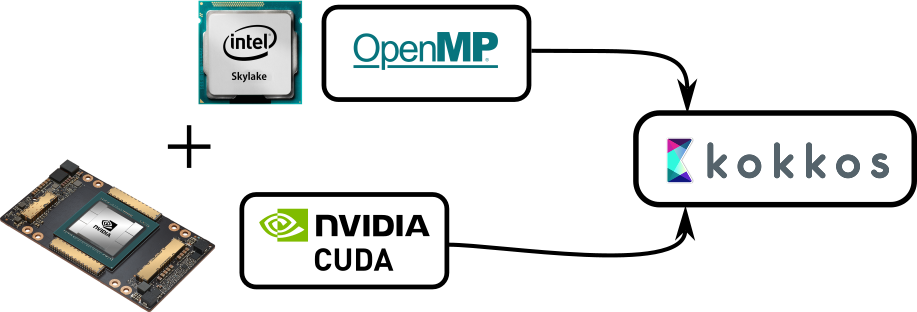
\includegraphics[width=\textwidth]{kokkos_a100_compilation.png}
            \end{center}
            \begin{minted}{sh}
                cmake \
                    -B ${build_dir} \
                    -DKokkos_ENABLE_OPENMP=ON \
                    -DKokkos_ARCH_SKX=ON \
                    -DKokkos_ENABLE_CUDA=ON \
                    -DKokkos_ARCH_AMPERE80=ON
            \end{minted}
        \end{column}
        \begin{column}{0.525\linewidth}
            \begin{itemize}
                \item Compiling for a multi-core Xeon Skylake CPU and an NVIDIA A100 GPU
                \item Compiler is GCC (default)
                \item OpenMP option for the multi-core CPU
                \item Skylake option, mostly for vectorization (optional)
                \item Cuda option for the GPU
                \item A100 option, for the correct architecture (mandatory)
            \end{itemize}
        \end{column}
    \end{columns}
\end{frame}

\begin{frame}[fragile]{Real world case: AMD GPU}
    \begin{columns}
        \begin{column}{0.475\linewidth}
            \begin{center}
                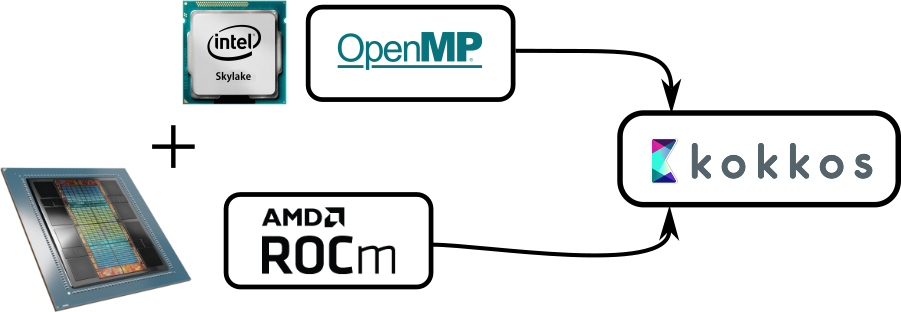
\includegraphics[width=\textwidth]{kokkos_mi300x_compilation.png}
            \end{center}
            \begin{minted}{sh}
                cmake \
                    -B ${build_dir} \
                    -DCMAKE_CXX_COMPILER=hipcc \
                    -DKokkos_ENABLE_OPENMP=ON \
                    -DKokkos_ARCH_SKX=ON \
                    -DKokkos_ENABLE_HIP=ON \
                    -DKokkos_ARCH_AMD_GFX90A=ON
            \end{minted}
        \end{column}
        \begin{column}{0.525\linewidth}
            \begin{itemize}
                \item Compiling for a multi-core Xeon Skylake CPU and an AMD MI300X GPU
                \item Compiler is the HIP compiler
                \item OpenMP option for the multi-core CPU
                \item Skylake option, mostly for vectorization (optional)
                \item HIP option for the GPU
                \item MI300X option, for the correct architecture (mandatory)
            \end{itemize}
        \end{column}
    \end{columns}
\end{frame}

\begin{frame}[fragile]{Real world case: Intel GPU}
    \begin{columns}
        \begin{column}{0.475\linewidth}
            \begin{center}
                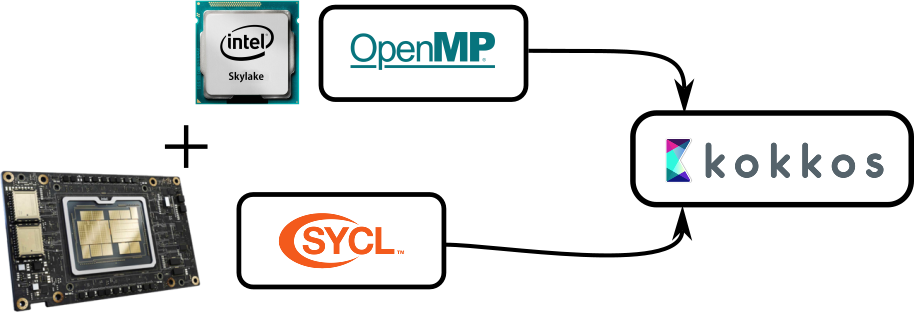
\includegraphics[width=\textwidth]{kokkos_gpu_max_compilation.png}
            \end{center}

            \vspace{-0.5em}

            \begin{minted}[breakafter={=}]{sh}
                cmake \
                    -B ${build_dir} \
                    -DCMAKE_CXX_COMPILER=icpx \
                    -DCMAKE_CXX_FLAGS="-fp-model=precise" \
                    -DKokkos_ENABLE_OPENMP=ON \
                    -DKokkos_ARCH_SKX=ON \
                    -DKokkos_ENABLE_SYCL=ON \
                    -DKokkos_ARCH_INTEL_PVC=ON
            \end{minted}
        \end{column}
        \begin{column}{0.525\linewidth}
            \begin{itemize}
                \item Compiling for a multi-core Xeon Skylake CPU and an Intel GPU Max
                \item Compiler is the Intel LLVM compiler
                \item Add flag to use high precision math operators
                \item OpenMP option for the multi-core CPU
                \item Skylake option, mostly for vectorization (optional)
                \item SYCL option for the GPU
                \item PVC option, for the correct architecture (mandatory)
            \end{itemize}
        \end{column}
    \end{columns}
\end{frame}

\begin{exerciseframe}{Build Kokkos for a GPU backend}
    \begin{columns}
        \begin{column}{0.475\linewidth}
            \begin{minted}[breakafter={=}]{sh}
                cmake \
                    -S /src/kokkos \
                    -B build/cuda \
                    -DCMAKE_BUILD_TYPE=Release \
                    -DKokkos_ENABLE_CUDA=ON \
                    -DKokkos_ARCH_XXX=ON

                cmake \
                    --build build/cuda \
                    --parallel 4

                cmake \
                    --install build/cuda \
                    --prefix $HOME/opt/kokkos/cuda
            \end{minted}
        \end{column}
        \begin{column}{0.525\linewidth}
            \begin{itemize}
                \item Build and install Kokkos with the CUDA backend
                \item Enable CUDA architecture \texttt{XXX} (not required if you are on a GPU node)
            \end{itemize}
            \vspace{1em}

            \begin{center}
                \scriptsize
                \begin{table}{Usual GPU architectures}{ll}
                    GPU model & Option \\\hline
                    AMD MI300A & \texttt{-DKokkos\_ARCH\_AMD\_GFX942\_APU=ON} \\
                    AMD MI300X & \texttt{-DKokkos\_ARCH\_AMD\_GFX942=ON} \\
                    AMD MI250X & \texttt{-DKokkos\_ARCH\_AMD\_GFX90A=ON} \\
                    NVIDIA H200 & \texttt{-DKokkos\_ARCH\_HOPPER90=ON} \\
                    NVIDIA A100 & \texttt{-DKokkos\_ARCH\_AMPERE80=ON} \\
                    NVIDIA V100 & \texttt{-DKokkos\_ARCH\_VOLTA70=ON}
                \end{table}
            \end{center}
        \end{column}
    \end{columns}
\end{exerciseframe}


\begin{exerciseframe}{From the "hello\_world" folder}
    \begin{columns}
        \begin{column}{0.5\linewidth}
            \begin{minted}[breakafter={=}]{sh}
                cmake \
                    -B build/serial \
                    -DCMAKE_BUILD_TYPE=Release \
                    -DKokkos_ROOT=$HOME/opt/kokkos/cuda

                cmake \
                    --build build/cuda
            \end{minted}
        \end{column}
        \begin{column}{0.5\linewidth}
            \begin{itemize}
                \item Build the hello world code
                \item Run with the \texttt{--kokkos-print-configuration} argument
            \end{itemize}
        \end{column}
    \end{columns}
\end{exerciseframe}

\begin{exerciseframe}{\small From last week worktree of the "cpu\_base" folder}
    \begin{columns}
        \begin{column}{0.55\linewidth}
            \begin{minted}[breakafter={=}]{sh}
                cmake \
                    -B build/cuda \
                    -DCMAKE_BUILD_TYPE=Release \
                    -DKokkos_ROOT=$HOME/opt/kokkos/cuda

                cmake \
                    --build build/cuda
            \end{minted}
        \end{column}
        \begin{column}{0.45\linewidth}
            \begin{itemize}
                \item Compile the CPU code with the CUDA backend
                \item Try to run it
            \end{itemize}

            \pause
            \vspace{1em}
            \begin{block}{Holly Molly}
                The program crashes!
            \end{block}
        \end{column}
    \end{columns}
\end{exerciseframe}

\section{About portability}

\begin{frame}[fragile]{Why do we need KOKKOS\_LAMBDA?}
    \begin{columns}
        \begin{column}{0.4\linewidth}
            \begin{minted}{C++}
                Kokkos::parallel_for(
                    "my_loop", N,
                    [=] (int i) {
                        A(i) = B(i) + C(i);
                    }
                );
            \end{minted}
            \begin{uncoverenv}<3->
                \begin{block}{Question}
                    Why do we need to use \texttt{KOKKOS\_LAMBDA} inside parallel constructs rather than the standard C++ lambda syntax?
                \end{block}
            \end{uncoverenv}
        \end{column}
        \begin{column}{0.6\linewidth}
            \begin{itemize}
                \item Let's create a \texttt{parallel\_for} without \texttt{KOKKOS\_LAMBDA}
                \item This code works when compiled with a CPU backend
                \pause
                \item But fails when compiled on CUDA backend with a cryptic error message:
                \begin{minted}[fontsize=\scriptsize]{text}
                    error: The closure type for a lambda ("lambda [](int)->void") cannot be used in the template argument type of a __global__ function template instantiation, unless the lambda is defined within a __device__ or __global__ function
                \end{minted}
            \end{itemize}
        \end{column}
    \end{columns}
\end{frame}

\begin{frame}[fragile]{Function annotations}
    \begin{columns}
        \begin{column}{0.47\linewidth}
            \begin{minted}{C++}
                __device__
                void device_function() {}

                __host__
                void host_function() {}

                __host__ __device__
                void host_device_function() {}

                auto lambda =
                  __host__ __device__ [] () {};
            \end{minted}
        \end{column}
        \begin{column}{0.55\linewidth}
            \begin{itemize}
                \item GPU backends need special annotation to know which code will be run on the host and which code will run on the device
                \item Lambdas also need to be annotated
                \item Function annotated with both \texttt{\_\_host\_\_} and \texttt{\_\_device\_\_} will be callable from the host and the device
                \item \texttt{\_\_host\_\_} is implicit if no annotation is given
                \item Neither \texttt{\_\_host\_\_} nor \texttt{\_\_device\_\_} are known by CPU backends, and will produce compilation errors
            \end{itemize}
        \end{column}
    \end{columns}
\end{frame}

\begin{frame}[fragile]{Annotated functions calls}
    \begin{center}
        \begin{table}{Effect of calling annotated functions}{l|lll}
            \diagbox[linecolor=darkmain,linewidth=0.5mm]{Caller}{Calling}& \texttt{\_\_host\_\_}  & \texttt{\_\_device\_\_} & both\\\hline
            \texttt{\_\_host\_\_} & Ok & Error & Ok \\
            \texttt{\_\_device\_\_} & Error & Ok & Ok \\
            both & Warning & Error & Ok
        \end{table}
    \end{center}
\end{frame}

\begin{frame}[fragile]{Kokkos annotation macros}
    \begin{columns}
        \begin{column}{0.45\linewidth}
            \begin{minted}{C++}
                KOKKOS_FUNCTION
                void device_function(){}

                KOKKOS_FUNCTION
                void host_function() {}

                KOKKOS_FUNCTION
                void host_device_function() {}

                auto lambda =
                KOKKOS_LAMBDA () {};
            \end{minted}
        \end{column}
        \begin{column}{0.55\linewidth}
            \begin{itemize}
                \item \texttt{KOKKOS\_FUNCTION} and \texttt{KOKKOS\_LAMBDA} will have the following annotations:
                \begin{itemize}
                    \item \texttt{\_\_host\_\_ \_\_device\_\_} when compiling for a GPU backend
                    \item Nothing when compiling for a CPU backend
                \end{itemize}
            \end{itemize}
        \end{column}
    \end{columns}
\end{frame}



\begin{frame}[fragile]{Annotated functions calls (with Kokkos macros)}
    \begin{center}
        \begin{table}{Effect of calling annotated functions}{l|lll}
            \diagbox[linecolor=darkmain,linewidth=0.5mm]{Caller}{Calling}& No macro  & \texttt{KOKKOS\_FUNCTION} & \texttt{KOKKOS\_LAMBDA} \\\hline
            No macro & Ok & Ok & Ok \\
            \texttt{KOKKOS\_FUNCTION} & Error & Ok & Ok \\
            \texttt{KOKKOS\_LAMBDA} & Error & Ok & Ok
        \end{table}
    \end{center}
\end{frame}

\begin{frame}[fragile]{Use of annotated functions in Kokkos}
    \begin{columns}
        \begin{column}{0.5\linewidth}
            \begin{minted}{C++}
                KOKKOS_FUNCTION
                int function(int i) {
                    // ...
                }

                void compute() {
                    Kokkos::parallel_for(
                        "compute",
                        N,
                        KOKKOS_LAMBDA (int i) {
                            int a = function(i);
                            // ...
                        }
                    );
                }
            \end{minted}
        \end{column}
        \begin{column}{0.5\linewidth}
            \begin{itemize}
                \item You already know where to use \texttt{KOKKOS\_LAMBDA}
                \pause
                \item \texttt{KOKKOS\_FUNCTION} can be used to create free functions called in a lambda
            \end{itemize}
        \end{column}
    \end{columns}
\end{frame}

\section{Memory spaces}

\begin{frame}{Where are a View data stored?}
    \begin{center}
        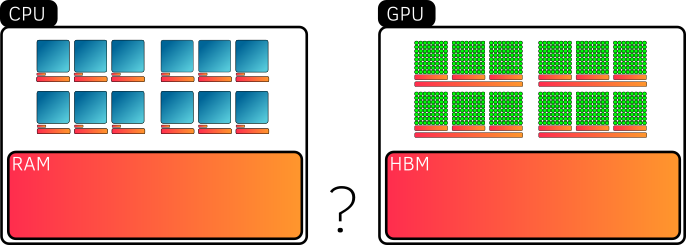
\includegraphics[width=0.6\textwidth]{view_memory.png}
    \end{center}
    \pause
    \begin{itemize}
        \item A View data is allocated only in one specific memory (Host or Device), never both
        \pause
        \item Suppose we created a view on the Host
    \end{itemize}
\end{frame}

\begin{frame}{Where are a View data stored? CPU version}
    \begin{center}
        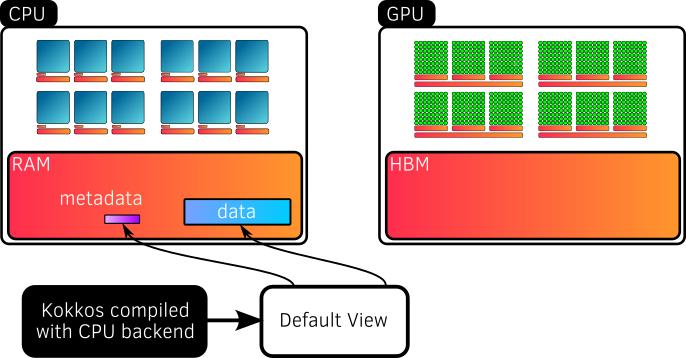
\includegraphics[width=0.6\textwidth]{host_view_memory.png}
    \end{center}
    \begin{itemize}
        \item If Kokkos is compiled with a \structure{CPU backend only}, the View data is allocated in the \structure{Host memory} by default
        \item View comes with metadata (number of dimensions, extents, etc.) and data
        \item Host view data usually \structure{cannot} be accessed from the Device
    \end{itemize}
\end{frame}

\begin{frame}{Where are a View data stored? GPU version}
    \begin{center}
        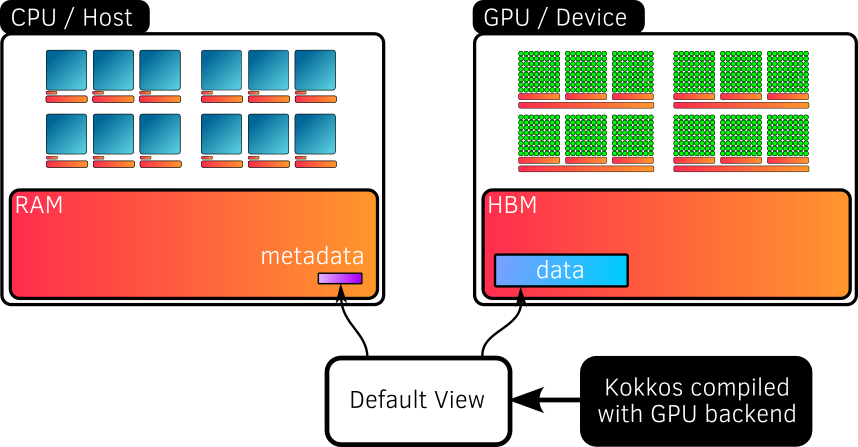
\includegraphics[width=0.6\textwidth]{device_view_memory.png}
    \end{center}

    \vspace{-1em}

    \begin{itemize}
        \item If Kokkos is compiled with a \structure{GPU backend}, the View data is allocated in the \structure{Device memory} by default
        \item Metadata are on the Host
        \item Device view data usually \structure{cannot} be accessed on the Host (we'll see later how to transfer data)
    \end{itemize}

    \vspace{0.5em}
\end{frame}

\begin{frame}{The concept of memory space}
    \begin{center}
        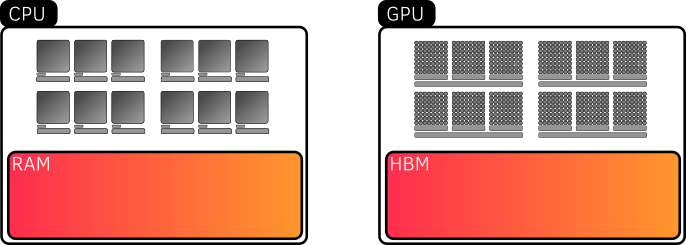
\includegraphics[width=0.6\linewidth]{memory_space.png}
    \end{center}
    \begin{itemize}
        \item Kokkos abstraction for where the data are allocated: \structure{memory space}
        \item A View is always associated, at compile time, to a specific memory space (Host or Device)
        \item By default, view data is allocated
        \begin{itemize}
            \item On the Host if no GPU backend is available
            \item On the Device otherwise
        \end{itemize}
    \end{itemize}
\end{frame}

\begin{frame}[fragile]{How to set a memory space}
    \begin{columns}
        \begin{column}{0.5\linewidth}
            \begin{minted}{C++}
                Kokkos::View<int**, MemorySpace>
                    my_matrix("matrix", 10, 10);
            \end{minted}
        \end{column}
        \begin{column}{0.5\linewidth}
            \begin{itemize}
                \item Template argument \texttt{MemorySpace} to specify the memory space when creating a view
                \item Several ones available
                \item Using a backend-specific memory space is possible, but it breaks portability
                \item Common values are usually sufficient for basic usages
            \end{itemize}
        \end{column}
    \end{columns}
\end{frame}

\begin{frame}{View with SharedSpace memory space}
    \begin{center}
        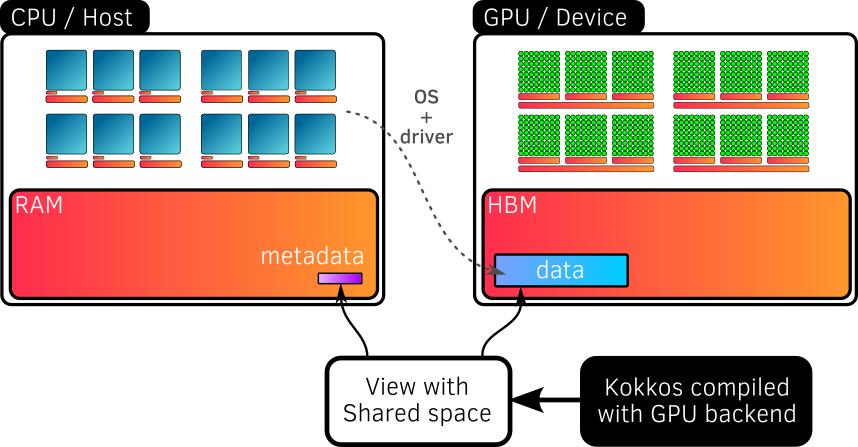
\includegraphics[width=0.6\textwidth]{shared_view_memory.png}
    \end{center}

    \vspace{-1em}

    \begin{itemize}
        \item If Kokkos is compiled with a \structure{GPU backend}, the View data is allocated in the \structure{Device memory}
        \item Shared view data \structure{can} be accessed from the Host by pages, which is managed by the OS and the driver
        \item Convenient, but comes with a slight performance cost
    \end{itemize}
\end{frame}

\begin{exerciseframe}{\small From your worktree of the "cpu\_base" folder}
    \begin{columns}
        \begin{column}{0.5\linewidth}
            \begin{minted}{C++}
                using View =
                    Kokkos::View<
                        double **,
                        Kokkos::SharedSpace
                    >;
            \end{minted}
        \end{column}
        \begin{column}{0.5\linewidth}
            \begin{itemize}
                \item Use the Kokkos \texttt{SharedSpace} memory space for the views
                \item Try to run the code
            \end{itemize}
            \pause
            \vspace{1em}
            \begin{block}{Holly Molly}
                The results are wrong!
            \end{block}
        \end{column}
    \end{columns}
\end{exerciseframe}

\section{Fencing}

\begin{frame}[fragile]{Asynchronous execution on GPU}
    \begin{columns}
        \begin{column}{0.5\linewidth}
            \begin{minted}{C++}
                // parallel loop on Device
                Kokkos::parallel_for(
                    "my_loop",
                    N,
                    KOKKOS_LAMBDA (int i) {
                        data(i) = // ...
                    }
                );

                // Host code
                host_function(data);
            \end{minted}
        \end{column}
        \begin{column}{0.5\linewidth}
            \begin{itemize}
                \item With a GPU backend, the parallel loop is executed asynchronously on the GPU
                \item The loop is launched and the program continues
                \item We will work with asynchronism this afternoon
            \end{itemize}

            \pause

            \begin{block}{Problem}
                What if I need the result of the parallel loop in the host code?
            \end{block}
        \end{column}
    \end{columns}
\end{frame}

\begin{frame}[fragile]{All you need is a fence}
    \begin{columns}
        \begin{column}{0.5\linewidth}
            \begin{minted}{C++}
                // parallel loop on Device
                Kokkos::parallel_for(
                    "my_loop",
                    N,
                    KOKKOS_LAMBDA (int i) {
                        data(i) = // ...
                    }
                );

                Kokkos::fence("my_loop fence");

                // Host code
                host_function(data);
            \end{minted}
        \end{column}
        \begin{column}{0.5\linewidth}
            \begin{itemize}
                \item \texttt{fence} to wait for asynchronous work to be completed
                \item Equivalent to OpenMP \texttt{barrier} or to \texttt{MPI\_Wait}
                \item Fence label (bonus for debugging!)
            \end{itemize}
        \end{column}
    \end{columns}
\end{frame}

\begin{exerciseframe}{\small From your worktree or the "gpu\_base\_0\_shared\_space" folder}
    \begin{columns}
        \begin{column}{0.5\linewidth}
            \begin{minted}{C++}
                Kokkos::parallel_for(
                    "my_loop",
                    N,
                    KOKKOS_LAMBDA (int i) {
                        // ...
                    }
                );

                Kokkos::fence("my_loop fence");
            \end{minted}
        \end{column}
        \begin{column}{0.5\linewidth}
            \begin{itemize}
                \item Use the Kokkos \texttt{fence} after the \texttt{parallel\_for}
                \item Try to run the code
            \end{itemize}
            \pause
            \vspace{0.5em}
            \begin{block}{Holly Molly}
                It works!
            \end{block}
            \pause
            \begin{itemize}
                \item Run with the parameter \texttt{-n 20}
            \end{itemize}
            \pause
            \vspace{0.5em}
            \begin{block}{Holly Molly}
                The results are wrong again!
            \end{block}
        \end{column}
    \end{columns}
\end{exerciseframe}

\section{Layout and iteration order}

\begin{frame}{Reminder about Views layout}
    \begin{center}
        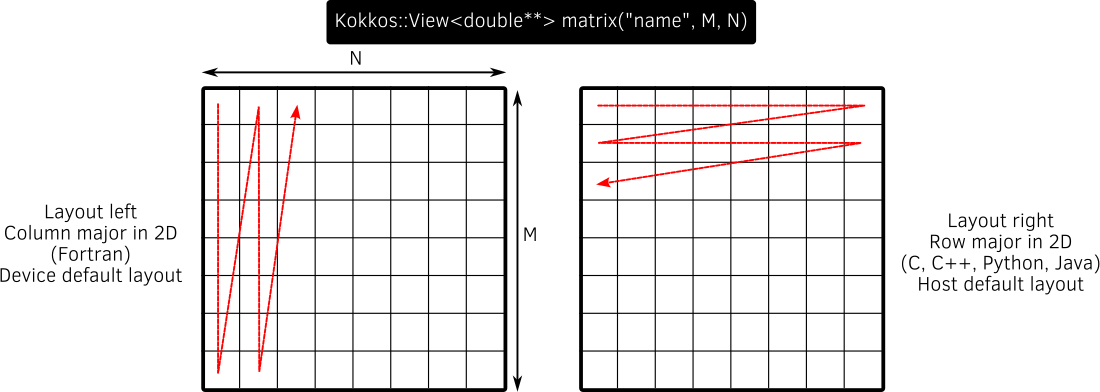
\includegraphics[width=0.75\textwidth]{layout_right_left.png}
    \end{center}
    \begin{itemize}
        \item Layout is the way multidimensional indices map to linear memory
        \item The default layout of a View depends on the backend
        \begin{itemize}
            \item Layout right on CPU
            \item Layout left on GPU
        \end{itemize}
        \item This means data dumped to a file will differ depending on the backend
    \end{itemize}
\end{frame}

\begin{frame}{Iteration order}
    \begin{center}
        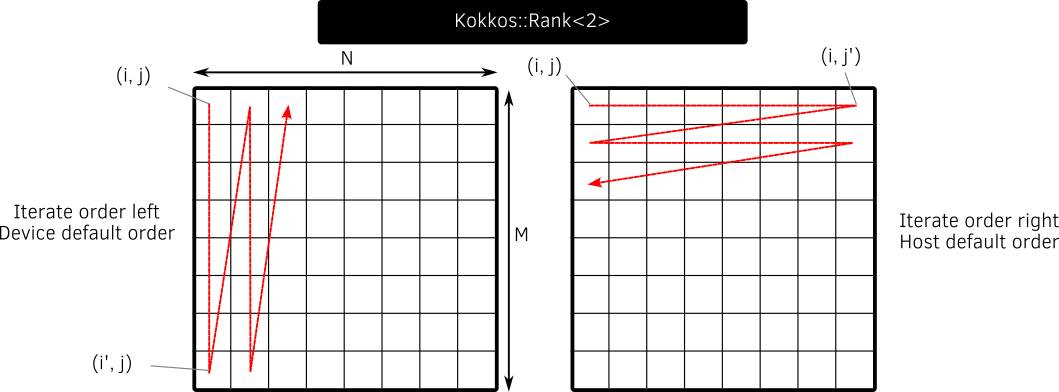
\includegraphics[width=0.75\textwidth]{iterate_right_left.png}
    \end{center}
    \begin{itemize}
        \item Iteration order is the way multidimensional indices are traversed by threads
        \item The default iterate order depends on the backend
        \begin{itemize}
            \item Order right on CPU
            \item Order left on GPU
        \end{itemize}
    \end{itemize}
\end{frame}

\begin{frame}[fragile]{Iteration order(s) for Kokkos}
    \begin{columns}
        \begin{column}{0.5\linewidth}
            \begin{minted}{C++}
                using Rank = Kokkos::Rank<
                    N,
                    // outer
                    Kokkos::Iterate::Default,
                    // inner
                    Kokkos::Iterate::Default
                >;
            \end{minted}
        \end{column}
        \begin{column}{0.5\linewidth}
            \begin{itemize}
                \item \texttt{Range} to specify the iteration order
                \item Kokkos iterates by tiles, so there are 2 iteration orders
                \begin{description}[Outer order]
                    \item[Outer order] Order of the tiles within the iteration space
                    \item[Inner order] Order within the tile
                \end{description}
                \item Possible values
                \begin{description}[\texttt{Default}]
                    \item[\texttt{Default}] Depends on the backend
                    \item[\texttt{Left}] Left order
                    \item[\texttt{Right}] Right order
                \end{description}
                \item For best performance, the inner iteration order must match the memory layout of the accessed views
            \end{itemize}
        \end{column}
    \end{columns}
\end{frame}

\begin{exerciseframe}{\small From your worktree or the "gpu\_base\_1\_fences" folder}
    \begin{columns}
        \begin{column}{0.5\linewidth}
            \begin{minted}[fontsize=\scriptsize]{C++}
                using View =
                    Kokkos::View<
                        double**,
                        Kokkos::LayoutRight
                    >;

                // ...

                Kokkos::parallel_for(
                    // ...
                    Kokkos::MDrangePolicy<
                        Kokkos::Range<
                            2,
                            Kokkos::Iterate::Default,
                            Kokkos::Iterate::Right
                        >
                    >(/* ... */),
                    // ...
                );
            \end{minted}
        \end{column}
        \begin{column}{0.5\linewidth}
            \begin{itemize}
                \item Use \texttt{Kokkos::LayoutRight} for the views
                \item Use \texttt{Kokkos::Iterate::Right} for the range policies
                \item Try to run the code with the parameter \texttt{-n 20}
            \end{itemize}
            \pause
            \vspace{1em}
            \begin{block}{Holly Molly}
                It works!
            \end{block}
        \end{column}
    \end{columns}
\end{exerciseframe}

\section{Kokkos tools}

\begin{frame}{What is this about?}
    \begin{columns}[T]
        \begin{column}{0.5\linewidth}
            \begin{center}
                \textbf{Debugging}
            \end{center}
            \begin{itemize}
                \item Errors may happen
                \item Print-debugging is cumbersome
                \item Developers need real tools
                \begin{itemize}
                    \item \texttt{gdb} (CPU)
                    \item \texttt{compute-sanitizer} (CUDA)
                    \item \texttt{cuda-gdb} (CUDA)
                    \item \texttt{rocgdb} (HIP)
                    \item ...
                \end{itemize}
                \item What can Kokkos do?
            \end{itemize}
        \end{column}
        \pause
        \begin{column}{0.5\linewidth}
            \begin{center}
                \textbf{Profiling}
            \end{center}
            \begin{itemize}
                \item You want to optimize real bottlenecks
                \item \texttt{time} has its limits
                \item You don't want to create timers by yourself
                \item Developers need real tools
                \begin{itemize}
                    \item \texttt{perf} (CPU)
                    \item VTune (CPU)
                    \item NSight Systems/Compute (CUDA)
                    \item \texttt{rocprofv2} (HIP)
                    \item ...
                \end{itemize}
                \item What can Kokkos do?
            \end{itemize}
        \end{column}
    \end{columns}
\end{frame}

\begin{frame}{Kokkos debugging and profiling tools at hand}
    \begin{columns}[T]
        \begin{column}{0.33\linewidth}
            \begin{center}
                \textbf{Kokkos}
            \end{center}
            \begin{itemize}
                \item KokkosP interface
                \item Profiling regions
            \end{itemize}
            \begin{block}{Note}
                Not actual tools, but used by other tools
            \end{block}
            \begin{block}{Remark}
                Same interface for debugging and profiling
            \end{block}
        \end{column}
        \pause
        \begin{column}{0.33\linewidth}
            \begin{center}
                \textbf{Kokkos tools}
            \end{center}
            \begin{itemize}
                \item Kernel logger
                \item Kernel timer
                \item Memory usage
                \item Memory events
                \item Space time stack
                \item VTune connector
                \item NVTX connector
                \item ROCTX connector
                \item ...
            \end{itemize}
        \end{column}
        \pause
        \begin{column}{0.33\linewidth}
            \begin{center}
                \textbf{Third-party tools}
            \end{center}
            \begin{itemize}
                \item VTune
                \item Nsight Systems
                \item Nsight Compute
                \item Tau
                \item Timemory
                \item Caliper
                \item HPCToolkit
                \item Apex
                \item ...
            \end{itemize}
        \end{column}
    \end{columns}
\end{frame}

\begin{frame}[fragile]{KokkosP interface}
    \begin{columns}
        \begin{column}{0.55\linewidth}
            \begin{minted}{C++}
                Kokkos::View<int *> view("view", N);

                Kokkos::parallel_for(
                    "compute",
                    N,
                    KOKKOS_LAMBDA(int i) {
                        view(i) = // ...
                    }
                );

                Kokkos::fence(
                    "wait for compute"
                );
            \end{minted}
        \end{column}
        \begin{column}{0.45\linewidth}
            \begin{itemize}
                \item Profiling tools interface
                \item Provided by Kokkos
                \item Hooks in Kokkos functions
                \begin{itemize}
                    \item Parallel constructs
                    \item Fences
                \end{itemize}
                \item Designed for other tools to use it
                \item Always available
                \item Really small overhead if no tools are used (check of a Boolean)
            \end{itemize}
        \end{column}
    \end{columns}
\end{frame}

\begin{frame}[fragile]{Profiling regions}
    \begin{columns}
        \begin{column}{0.5\linewidth}
            \begin{minted}{C++}
                Kokkos::Profiling::pushRegion(
                    "computation"
                );

                // ...

                Kokkos::Profiling::popRegion();
            \end{minted}
        \end{column}
        \begin{column}{0.5\linewidth}
            \begin{itemize}
                \item Provided by Kokkos
                \item No specific header needed
                \item Namespace \texttt{Kokkos::Profiling}
                \item Set regions of interest in your code
                \begin{itemize}
                    \item \texttt{pushRegion} to start a region
                    \item \texttt{popRegion} to end a region
                \end{itemize}
                \item Regions can be nested
            \end{itemize}
        \end{column}
    \end{columns}
\end{frame}

\begin{frame}[fragile]{Profiling regions (RAII)}
    \begin{columns}
        \begin{column}{0.65\linewidth}
            \begin{minted}{C++}
                #include <Kokkos_Profiling_ScopedRegion.hpp>

                // ...

                {
                    Kokkos::Profiling::ScopedRegion
                        region("computation");

                    // ...
                }
            \end{minted}
        \end{column}
        \begin{column}{0.35\linewidth}
            \begin{itemize}
                \item Provided by Kokkos
                \item Specific header needed
                \item \texttt{ScopedRegion} is a class that ensures that \texttt{pushRegion} and \texttt{popRegion} are called correctly
                \item Set region for a scope
            \end{itemize}
        \end{column}
    \end{columns}
\end{frame}

\begin{frame}{Kokkos tools}
    \begin{itemize}
        \item Library of the Kokkos ecosystem
        \item \url{https://github.com/kokkos/kokkos-tools}
        \item \url{https://github.com/kokkos/kokkos-tools/wiki}
        \item Has a different version number than Kokkos
        \item Should be built and installed somewhere (this requires to install Kokkos too)
        \item You should update the environment variables \texttt{PATH} and \texttt{LD\_LIBRARY\_PATH}
        \item Use one tool at a time with either
        \begin{itemize}
            \item The environment variable \texttt{KOKKOS\_TOOLS\_LIBS}

            Mind the \texttt{S}!
            \item The \texttt{--kokkos-tools-libs} argument of the program

            Mind the \texttt{s}!
        \end{itemize}
        \item Do not ship it within your program (this is a dev tool!)
    \end{itemize}
\end{frame}

\begin{frame}[fragile]{Guided tour for a dummy code}
    \begin{columns}
        \begin{column}{0.67\linewidth}
            \begin{minted}{C++}
                Kokkos::Profiling::pushRegion("computation");

                Kokkos::View<int *> view("view", N);

                Kokkos::parallel_for(
                    "compute",
                    N,
                    KOKKOS_LAMBDA(int i) {
                        view(i) = i;
                    }
                );

                Kokkos::fence("wait for compute");

                Kokkos::Profiling::popRegion();
            \end{minted}
        \end{column}
        \begin{column}{0.3\linewidth}
            \begin{itemize}
                \item Very simple code
                \item Let's try some tools on it
            \end{itemize}
        \end{column}
    \end{columns}
\end{frame}

\begin{frame}[fragile]{Simple kernel logger for a basic debugging}
    \begin{columns}
        \begin{column}{0.6\linewidth}
            \begin{minted}[breakafter={=}]{sh}
                ./my_program \
                    --kokkos-tools-libs=libkp_kernel_logger.so
            \end{minted}

            \begin{minted}{text}
                KokkosP: Kernel Logger Library Initialized (sequence is 0, version: 20240906)
            \end{minted}
        \end{column}
        \begin{column}{0.4\linewidth}
            \begin{itemize}
                \item Simple tool for a basic logging of your program's Kokkos-related activity
                \item Run the program with the argument
                \item Run for a few number of iterations if possible
                \item When loaded, a tool always print something on screen
            \end{itemize}
        \end{column}
    \end{columns}
\end{frame}

\begin{frame}[fragile]{Simple kernel logger output}
    \begin{minted}[fontsize=\tiny]{text}
        KokkosP: Entering profiling region: computation
        KokkosP: Allocate<Cuda> name: view pointer: 0x7c67126aa000 size: 80000
        KokkosP: Executing fence on device 33554433 with unique execution identifier 0
        KokkosP: computation
        KokkosP:       SharedAllocationRecord<Kokkos::CudaSpace, void>::SharedAllocationRecord(): fence after copying header from HostSpace
        KokkosP: Execution of fence 0 is completed.
        KokkosP: Executing parallel-for kernel on device 33554433 with unique execution identifier 1
        KokkosP: computation
        KokkosP:       Kokkos::View::initialization [view] via memset
        KokkosP: Execution of kernel 1 is completed.
        KokkosP: Executing fence on device 33554433 with unique execution identifier 2
        KokkosP: computation

        ...

        KokkosP: Kokkos library finalization called.
    \end{minted}

    \begin{itemize}
        \item All Kokkos activity listed (parallel constructs, fences, View creations...)
        \item Useful for tracking chaining of kernels
        \item Difficult to read for long executions or when the kernels are asynchronous
        \item Good idea to redirect the output to a file
    \end{itemize}
\end{frame}

\begin{frame}[fragile]{Simple kernel timer for a basic profiling}
    \begin{columns}
        \begin{column}{0.6\linewidth}
            \begin{minted}[breakafter={=}]{sh}
                ./my_program \
                    --kokkos-tools-libs=libkp_kernel_timer.so
            \end{minted}

            \usemintedstyle{vim}
            \begin{minted}{text}
                KokkosP: Simple Kernel Timer Library Initialized (sequence is 0, version: 20240906)
                ...
                KokkosP: Kernel timing written to /path/to/name_of_report.dat
            \end{minted}

            \begin{minted}{sh}
                kp_reader ./name_of_report.dat
            \end{minted}
        \end{column}
        \begin{column}{0.4\linewidth}
            \begin{itemize}
                \item Simple tool for a basic timing analysis
                \item Run the program with the argument
                \item Analyze the generated data with the provided \texttt{kp\_reader} program
            \end{itemize}
        \end{column}
    \end{columns}
\end{frame}

\begin{frame}[fragile]{Simple kernel timer output}
    \begin{minted}{text}
        (Type)   Total Time, Call Count, Avg. Time per Call, %Total Time in Kernels, %Total Program Time
        -------------------------------------------------------------------------
        Regions:
        ...
        -------------------------------------------------------------------------
        Kernels:
        ...
        -------------------------------------------------------------------------
        Summary:
        ...
        -------------------------------------------------------------------------
    \end{minted}
    \begin{itemize}
        \item 3 sections in the report
        \item Let's analyze them
    \end{itemize}
\end{frame}

\begin{frame}[fragile]{Simple kernel timer output (for summary)}
    \begin{minted}{text}
        (Type)   Total Time, Call Count, Avg. Time per Call, %Total Time in Kernels, %Total Program Time
        -------------------------------------------------------------------------
        Summary:

        Total Execution Time (incl. Kokkos + non-Kokkos):                   0.00038 seconds
        Total Time in Kokkos kernels:                                       0.00030 seconds
        -> Time outside Kokkos kernels:                                  0.00008 seconds
        -> Percentage in Kokkos kernels:                                   78.75 %
        Total Calls to Kokkos Kernels:                                            2

        -------------------------------------------------------------------------
    \end{minted}
    \begin{itemize}
        \item Global metrics of the execution of the program
        \item Example for a very simple code
    \end{itemize}
\end{frame}

\begin{frame}[fragile]{Simple kernel timer output (for regions)}
    \begin{minted}{text}
        (Type)   Total Time, Call Count, Avg. Time per Call, %Total Time in Kernels, %Total Program Time
        -------------------------------------------------------------------------

        Regions:

        - computation
        (REGION)   0.000349 1 0.000349 117.590361 92.599620
    \end{minted}

    \begin{itemize}
        \item Regions are named after what you set in \texttt{pushRegion}
        \item Descending order of cumulated duration
        \item One set of two lines per region
    \end{itemize}
\end{frame}

\begin{frame}[fragile]{Simple kernel timer output (for kernels)}
    \begin{minted}{text}
        (Type)   Total Time, Call Count, Avg. Time per Call, %Total Time in Kernels, %Total Program Time

        -------------------------------------------------------------------------
        Kernels:

        - compute
        (ParFor)   0.000282 1 0.000282 94.939759 74.762808
        - Kokkos::View::initialization [view] via memset
        (ParFor)   0.000015 1 0.000015 5.060241 3.984820
    \end{minted}

    \begin{itemize}
        \item Kernels are named after what you set in parallel constructs (\texttt{parallel\_*})
        \item Some internal kernels are visible: Views initialization
        \item Descending order of cumulated duration
        \item One set of two lines per kernel
    \end{itemize}
\end{frame}

\begin{frame}{NVTX connector for NVIDIA tools}
    \begin{itemize}
        \item Simple connector to convert Kokkos named regions/kernels into NVTX regions
        \item NVIDIA Tools eXtension
        \item For NVIDIA tools
        \begin{itemize}
            \item Nsight Systems
            \item Nsight Compute
        \end{itemize}
        \item Lot of documentation about how to use these tools right
        \item Equivalent ROCTX connector for AMD
    \end{itemize}
\end{frame}

\begin{frame}[fragile]{NVTX connector and Nsight Systems}
    \begin{columns}
        \begin{column}{0.6\linewidth}
            \begin{minted}[breakafter={=}]{sh}
                nsys profile \
                    -o report \
                    ./my_program \
                        --kokkos-tools-libs=libkp_nvtx_connector.so
            \end{minted}

            \begin{minted}{text}
                KokkosP: NVTX Analyzer Connector (sequence is 0, version: 20240906)
            \end{minted}

            \begin{minted}{sh}
                nsys-ui report.nsys-rep
            \end{minted}
        \end{column}
        \begin{column}{0.4\linewidth}
            \begin{itemize}
                \item Analyze a program as a whole
                \item Run the program with the argument through \texttt{nsys}
                \item Do not run your program for too long when profiling!
                \item About 10 iterations is enough
                \item Open the generated report
            \end{itemize}
        \end{column}
    \end{columns}
\end{frame}

\begin{frame}{Nsight Systems overview}
    \begin{columns}
        \begin{column}{0.75\linewidth}
            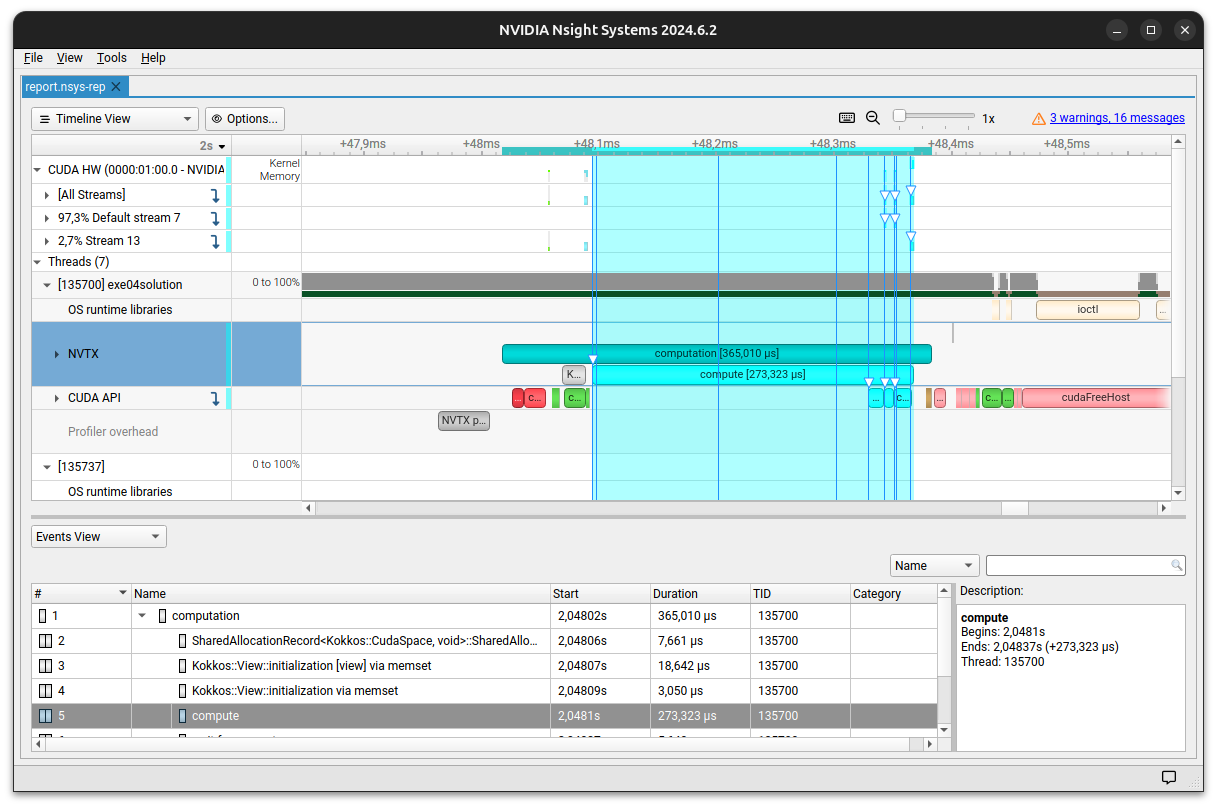
\includegraphics[width=\linewidth]{nsight_systems_example}
        \end{column}
        \begin{column}{0.25\linewidth}
            \begin{itemize}
                \item Activity against execution time
                \item Cuda activity
                \begin{itemize}
                    \item Kernels
                    \item Memory
                \end{itemize}
                \item NVTX
                \begin{itemize}
                    \item Parallel constructs
                    \item Fences
                    \item Regions
                \end{itemize}
                \item Cuda API calls
            \end{itemize}
        \end{column}
    \end{columns}
\end{frame}

\begin{frame}{Display NVTX name of kernels in Nsight Systems}
    \begin{columns}
        \begin{column}{0.5\linewidth}
            \begin{itemize}
                \item Kernels are named after function name, which for Kokkos is an obscure internal name
                \item Set to rename the kernels after the NVTX name
                \begin{enumerate}
                    \item Tools $\rightarrow$ Options
                    \item Behavior $\rightarrow$ Report
                    \item Set "Rename CUDA Kernels by NVTX" to \emph{Yes}
                    \item Re-open the report
                \end{enumerate}
            \end{itemize}
        \end{column}
        \begin{column}{0.5\linewidth}
            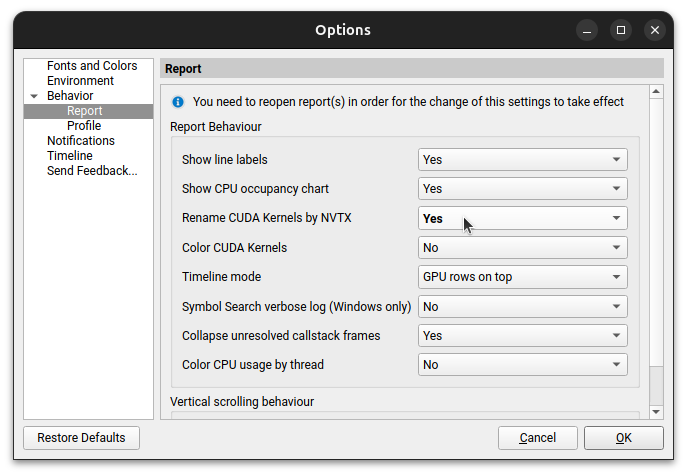
\includegraphics[width=\linewidth]{nsight_systems_options}
        \end{column}
    \end{columns}
\end{frame}

\begin{frame}[fragile]{NVTX connector and Nsight Compute}
    \begin{columns}
        \begin{column}{0.6\linewidth}
            \begin{minted}[breakafter={=}]{sh}
                ncu \
                    -o report \
                    --nvtx \
                    --nvtx-include "<NVTX region>/" \
                    --set detailed \
                    ./my_program \
                        --kokkos-tools-libs=libkp_nvtx_connector.so
            \end{minted}

            \begin{minted}{text}
                KokkosP: NVTX Analyzer Connector (sequence is 0, version: 20240906)
            \end{minted}

            \begin{minted}{sh}
                ncu-ui report.ncu-rep
            \end{minted}
        \end{column}
        \begin{column}{0.4\linewidth}
            \begin{itemize}
                \item Kernel by kernel analysis
                \item Run the program with the argument through \texttt{ncu}
                \item Use NVTX region to profile only certain kernels
                \item Set of metrics to collect
                \item The more the metrics, the slower the profiling
                \item Run for about 10 iterations
                \item Open the generated report
            \end{itemize}
        \end{column}
    \end{columns}
\end{frame}

\begin{frame}{Nsight Compute overview}
    \begin{columns}
        \begin{column}{0.75\linewidth}
            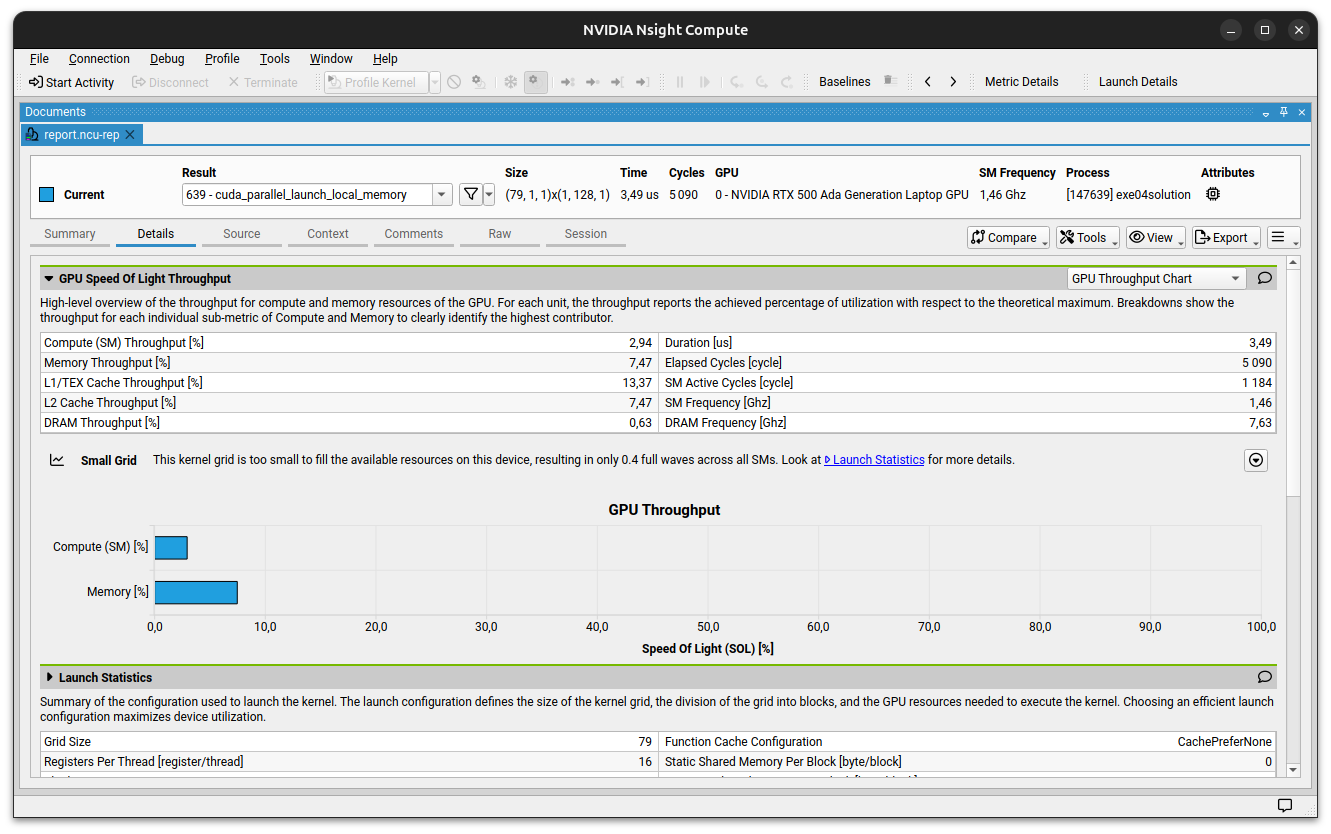
\includegraphics[width=\linewidth]{nsight_compute_example}
        \end{column}
        \begin{column}{0.25\linewidth}
            \begin{itemize}
                \item Details of each kernel
                \item Many metrics
                \begin{itemize}
                    \item Speed of light
                    \item Occupancy
                    \item ...
                \end{itemize}
                \item Can give suggestions
                \item Check online resources!
            \end{itemize}
        \end{column}
    \end{columns}
\end{frame}

\begin{exerciseframe}{Build Kokkos-Tools}
    \begin{columns}
        \begin{column}{0.6\linewidth}
            \begin{minted}[breakafter={=,/}, fontsize=\scriptsize]{C++}
                cmake \
                    -S /src/kokkos-tools \
                    -B build/cuda \
                    -DCMAKE_BUILD_TYPE=Release \
                    -DKokkos_ROOT=$HOME/opt/kokkos/cuda

                cmake \
                    --build build/cuda \
                    --parallel 4

                cmake \
                    --install build/cuda \
                    --prefix $HOME/opt/kokkos_tools/cuda

                export PATH=$HOME/opt/kokkos_tools/cuda/bin:$PATH
                export LD_LIBRARY_PATH=$HOME/opt/kokkos_tools/cuda/lib:$LD_LIBRARY_PATH
            \end{minted}
        \end{column}
        \begin{column}{0.4\linewidth}
            \begin{itemize}
                \item Build and install Kokkos-Tools for the installed instance of Kokkos
                \item Adjust the \texttt{PATH} and \texttt{LD\_LIBRARY\_PATH} environment variables
            \end{itemize}
        \end{column}
    \end{columns}
\end{exerciseframe}

\begin{exerciseframe}{\small From your worktree or the "gpu\_base\_2\_layout\_iterate" folder}
    \begin{columns}
        \begin{column}{0.5\linewidth}
            \begin{minted}{C++}
                Kokkos::Profiling::pushRegion(
                    "region name"
                );

                // ...

                Kokkos::Profiling::popRegion();
            \end{minted}

            \begin{minted}[breakafter={=}]{sh}
                nsys profile \
                    -o report \
                    ./my_program \
                        --kokkos-tools-libs=libkp_nvtx_connector.so

                nsys-ui report.nsys-rep
            \end{minted}
        \end{column}
        \begin{column}{0.5\linewidth}
            \begin{itemize}
                \item Add regions in the code and profile it
                \item Build the code with the OpenMP backend and compare (if you have time)
                \item Observe the performance with Nsight Systems
            \end{itemize}

            \pause
            \vspace{1em}
            \begin{block}{Holly Molly}
                This is not great
            \end{block}
        \end{column}
    \end{columns}
\end{exerciseframe}

\section{Explicit memory management}

\begin{frame}{How to access data living on the Device from the Host?}
    \begin{center}
        \includegraphics<1|handout:0>[width=0.9\textwidth]{device_memory_access_1.png}
        \includegraphics<2>[width=0.9\textwidth]{device_memory_access_2.png}
    \end{center}

    \begin{uncoverenv}<2>
        \begin{block}{Problem}
            You cannot!
        \end{block}
    \end{uncoverenv}
\end{frame}

\begin{frame}[fragile]{All you need is a mirror}
    \begin{columns}
        \begin{column}{0.6\linewidth}
            \begin{minted}{C++}
                Kokkos::View<int**>
                    device_matrix("matrix", 10, 10);

                auto host_matrix =
                    Kokkos::create_mirror_view(
                        device_matrix
                    );
            \end{minted}

        \end{column}
        \begin{column}{0.4\linewidth}
            \begin{itemize}
                \item A \structure{mirror} is a view in a different memory space
                \item Similar to its original view for the rest (shape, layout, etc.)
                \item \texttt{create\_mirror\_view} to create a mirror of a Device view on the Host
                \item If the original view is already on the Host (CPU backend), it creates a mirror without allocating memory (shallow copy of the original view)
                \item It allocates the memory but it \structure{doesn't copy the data}!
            \end{itemize}
        \end{column}
    \end{columns}
\end{frame}

\begin{frame}{How to access data living on the Device from the Host?}
    \begin{center}
        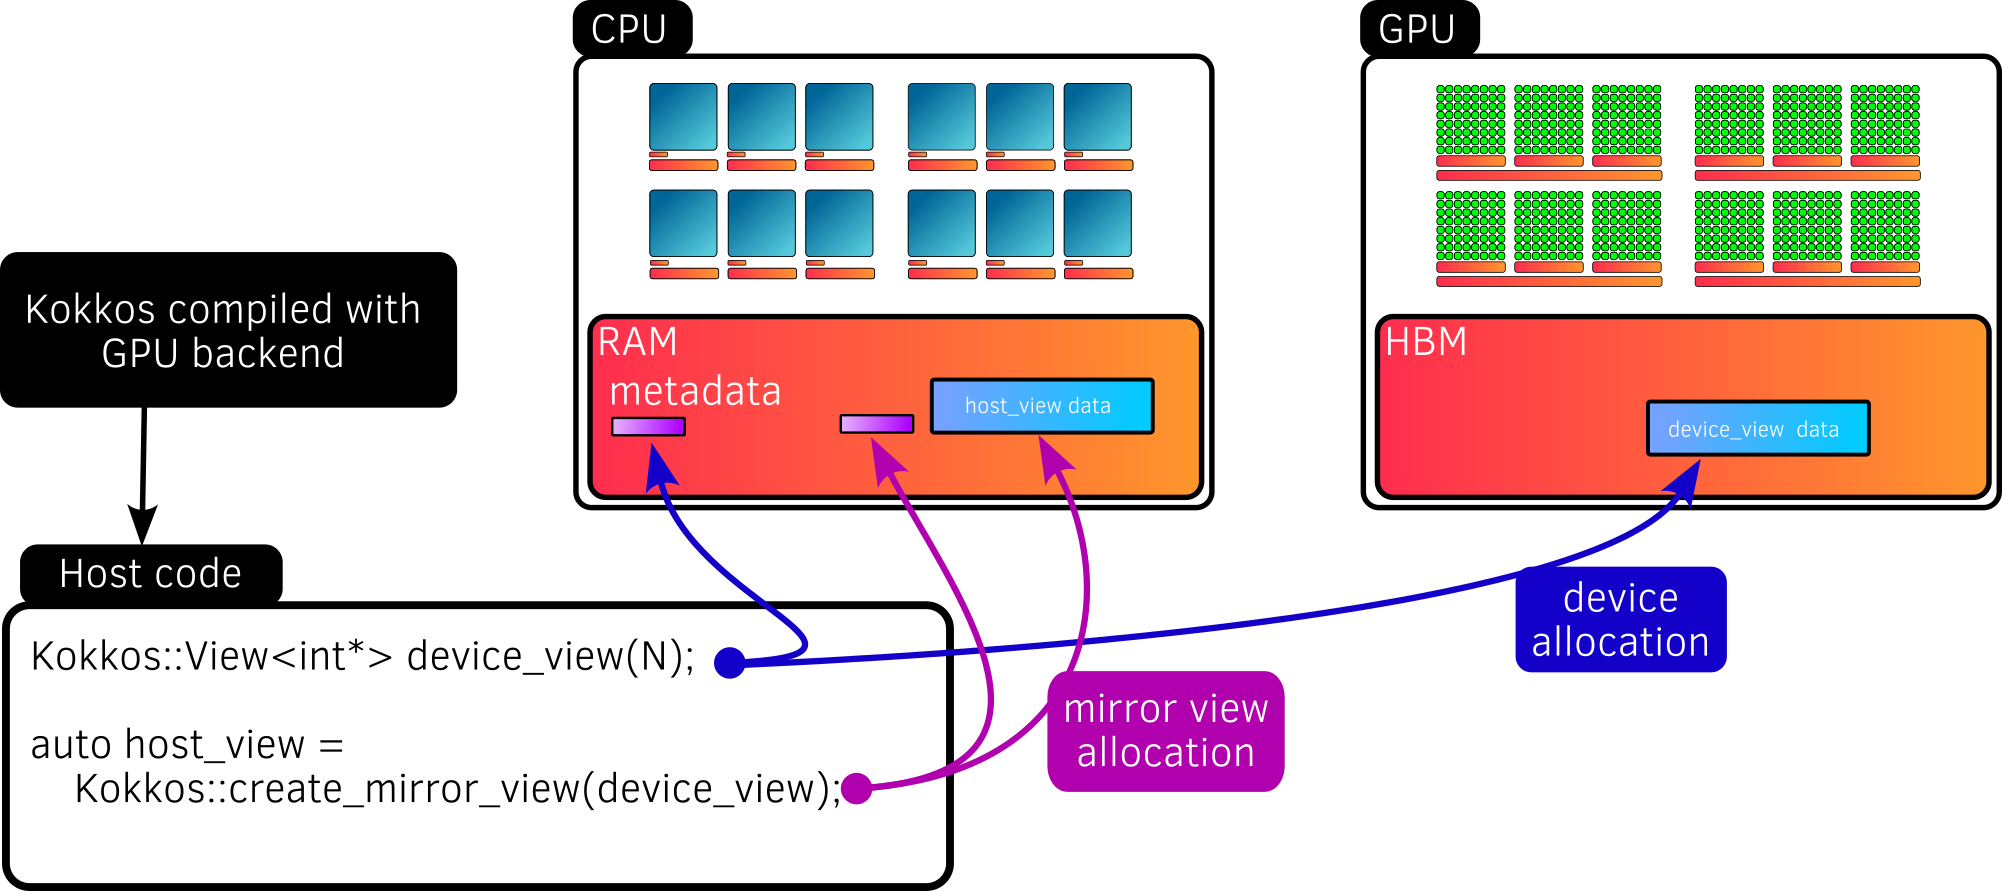
\includegraphics[width=0.9\textwidth]{device_mirror_view.png}
    \end{center}
\end{frame}

\begin{frame}{How to access data living on the Host from the Host?}
    \begin{center}
        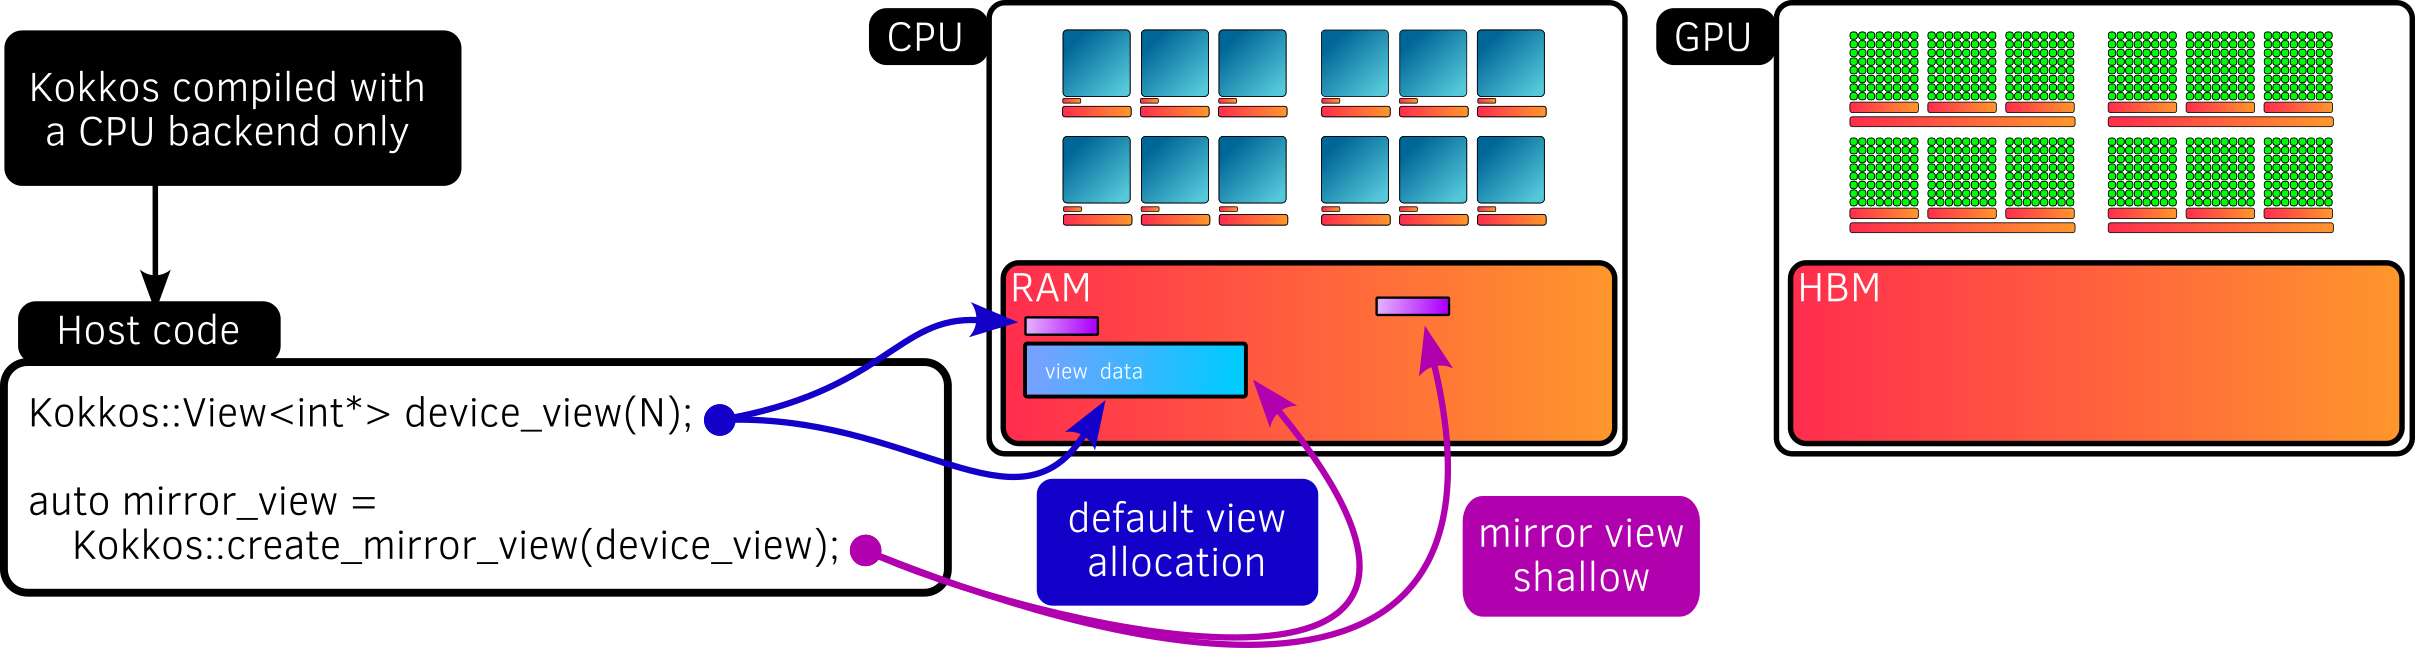
\includegraphics[width=0.9\textwidth]{host_create_mirror_view.png}
    \end{center}

    \begin{block}{Note}
        For portability reason, we always use a mirror view whether we compile with a CPU or GPU backend
    \end{block}
\end{frame}

\begin{frame}[fragile]{Deep copy data between memory spaces}
    \begin{columns}
        \begin{column}{0.5\linewidth}
            \begin{minted}{C++}
                Kokkos::View<int**>
                    device_view("view", Nx, Ny);

                auto host_view =
                    Kokkos::create_mirror_view(
                        device_view
                    );

                initialize(host_view);

                // from Host to Device
                Kokkos::deep_copy(
                    device_view,
                    host_view
                );
            \end{minted}
        \end{column}
        \begin{column}{0.5\linewidth}
            \begin{itemize}
                \item \texttt{deep\_copy(destination, source)} copy \texttt{source} to \texttt{destination}, even if the data are in different memory spaces
                \item Beware of \structure{arguments order!}
                \item Views must be similar (same shape, layout, etc.)
                \item If \texttt{deep\_copy} detects that the destination view is a shallow copy of the source view, it does nothing
            \end{itemize}
        \end{column}
    \end{columns}
\end{frame}

\begin{frame}{How to deep copy between the Host and the Device?}
    \begin{center}
        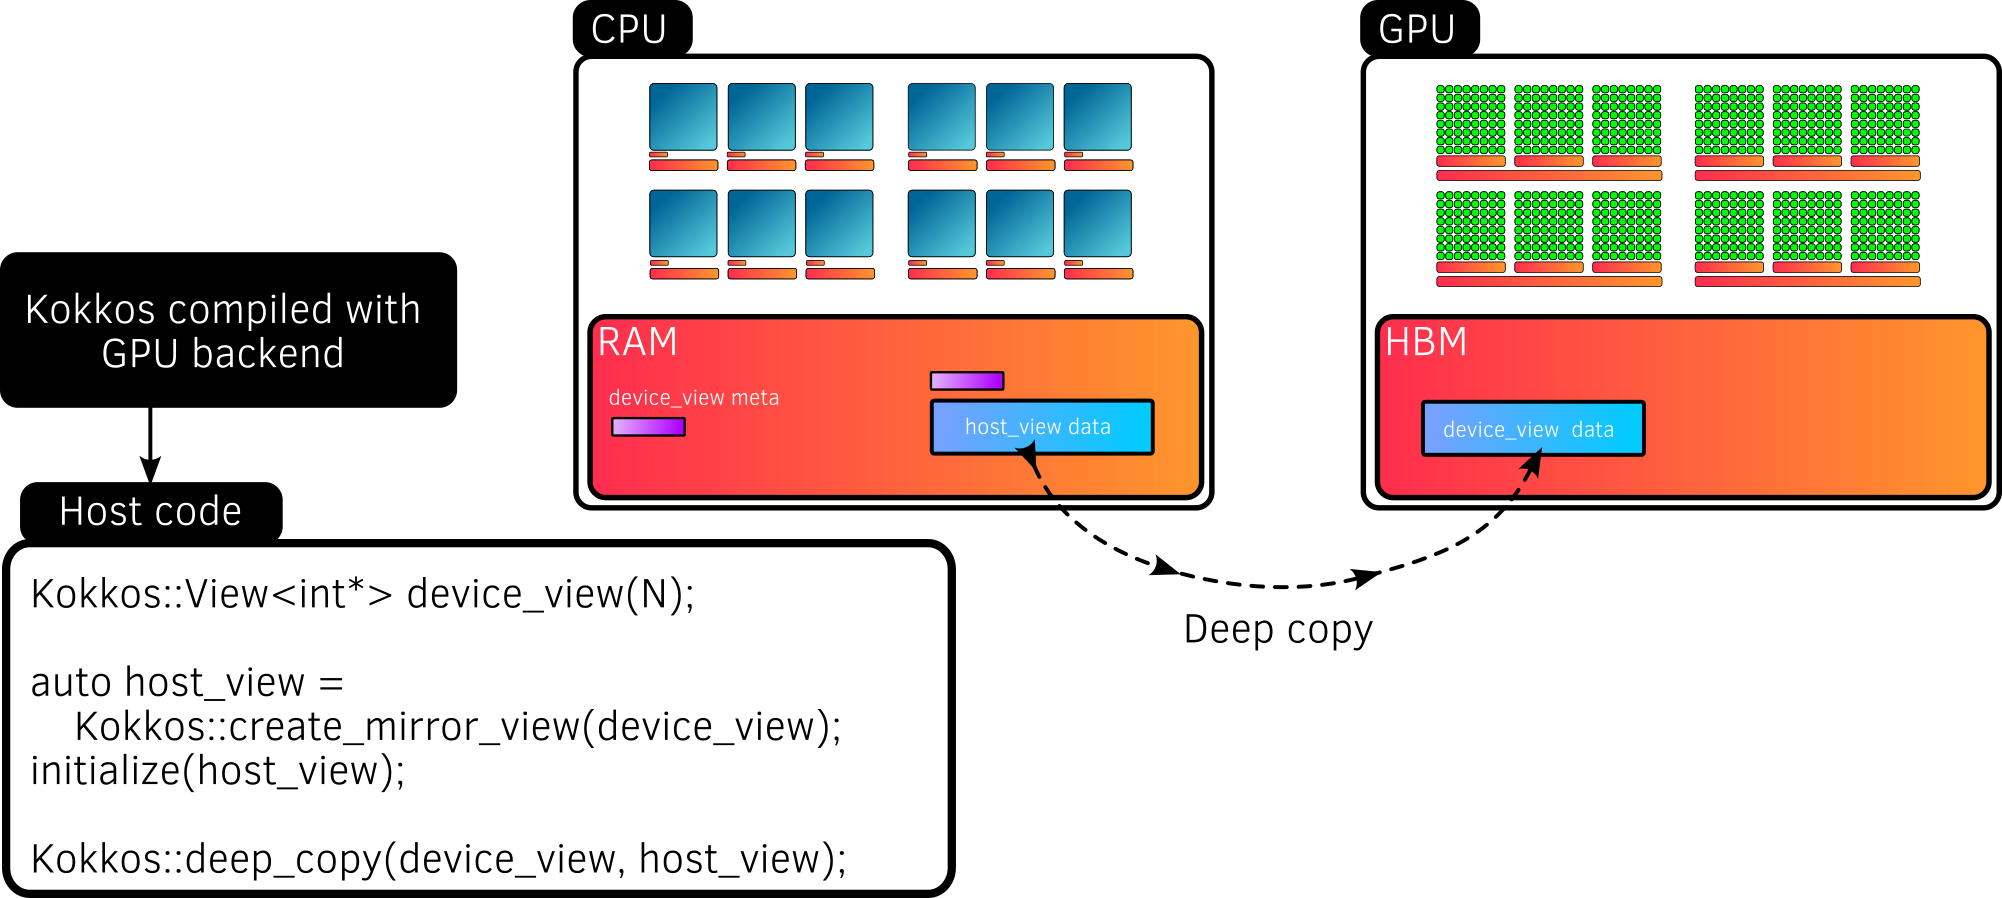
\includegraphics[width=0.9\textwidth]{host_device_deep_copy.png}
    \end{center}
\end{frame}

\begin{exerciseframe}{\small From your worktree or the "gpu\_base\_2\_layout\_iterate" folder}
    \begin{columns}
        \begin{column}{0.5\linewidth}
            \begin{minted}{C++}
                auto host_view =
                    Kokkos::create_mirror_view(
                        device_view
                    );

                // ...

                Kokkos::deep_copy(
                    device_view,
                    host_view
                );
            \end{minted}
        \end{column}
        \begin{column}{0.5\linewidth}
            \begin{itemize}
                \item Remove the \texttt{SharedSpace} memory space parameter of the views
                \item Add mirrors with Kokkos \texttt{create\_mirror\_view}
                \item Synchronize views and mirrors with \texttt{deep\_copy}
                \item Observe the performance with Nsight Systems
            \end{itemize}
        \end{column}
    \end{columns}
\end{exerciseframe}

\section{Execution spaces}

\begin{frame}{Now, where is my parallel loop executed?}
    \begin{center}
        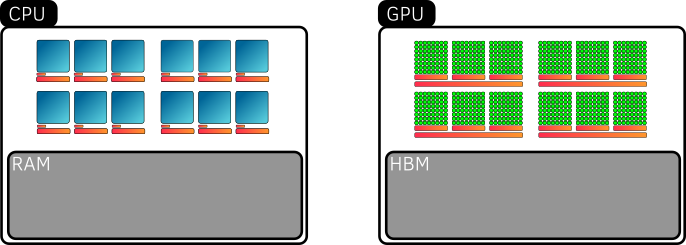
\includegraphics[width=0.8\linewidth]{execution_space.png}
    \end{center}
    \begin{itemize}
        \item Kokkos abstraction for where the loop is executed : \structure{execution space}
        \pause
        \item Parallel code (i.e. inside a \texttt{parallel\_*}) is by default executed
        \begin{itemize}
            \item By the Host if no GPU backend is available
            \item By the Device otherwise
        \end{itemize}
        \pause
        \item Serial code (the rest) is always executed on the Host
    \end{itemize}
\end{frame}

\begin{frame}{Execution space}
    \begin{itemize}
        \item Execution space to control where the loop is executed (CPU or GPU)
        \item Several ones available
        \item \texttt{Kokkos::DefaultExecutionSpace} and \texttt{Kokkos::DefaultHostExecutionSpace} are enough for beginners
        \item Using a backend-specific execution space is possible, but it breaks portability
    \end{itemize}
    \pause
    \begin{center}
        \begin{table}{Default execution spaces}{lll}
            & \multicolumn{2}{l}{Kokkos compiled on} \\
            Execution space & CPU backend & GPU backend \\\hline
            \texttt{Kokkos::DefaultExecutionSpace} & On CPU & On GPU \\
            \texttt{Kokkos::DefaultHostExecutionSpace} & On CPU & On CPU
        \end{table}
    \end{center}
\end{frame}

\begin{frame}{Default execution space summary}
    \begin{center}
        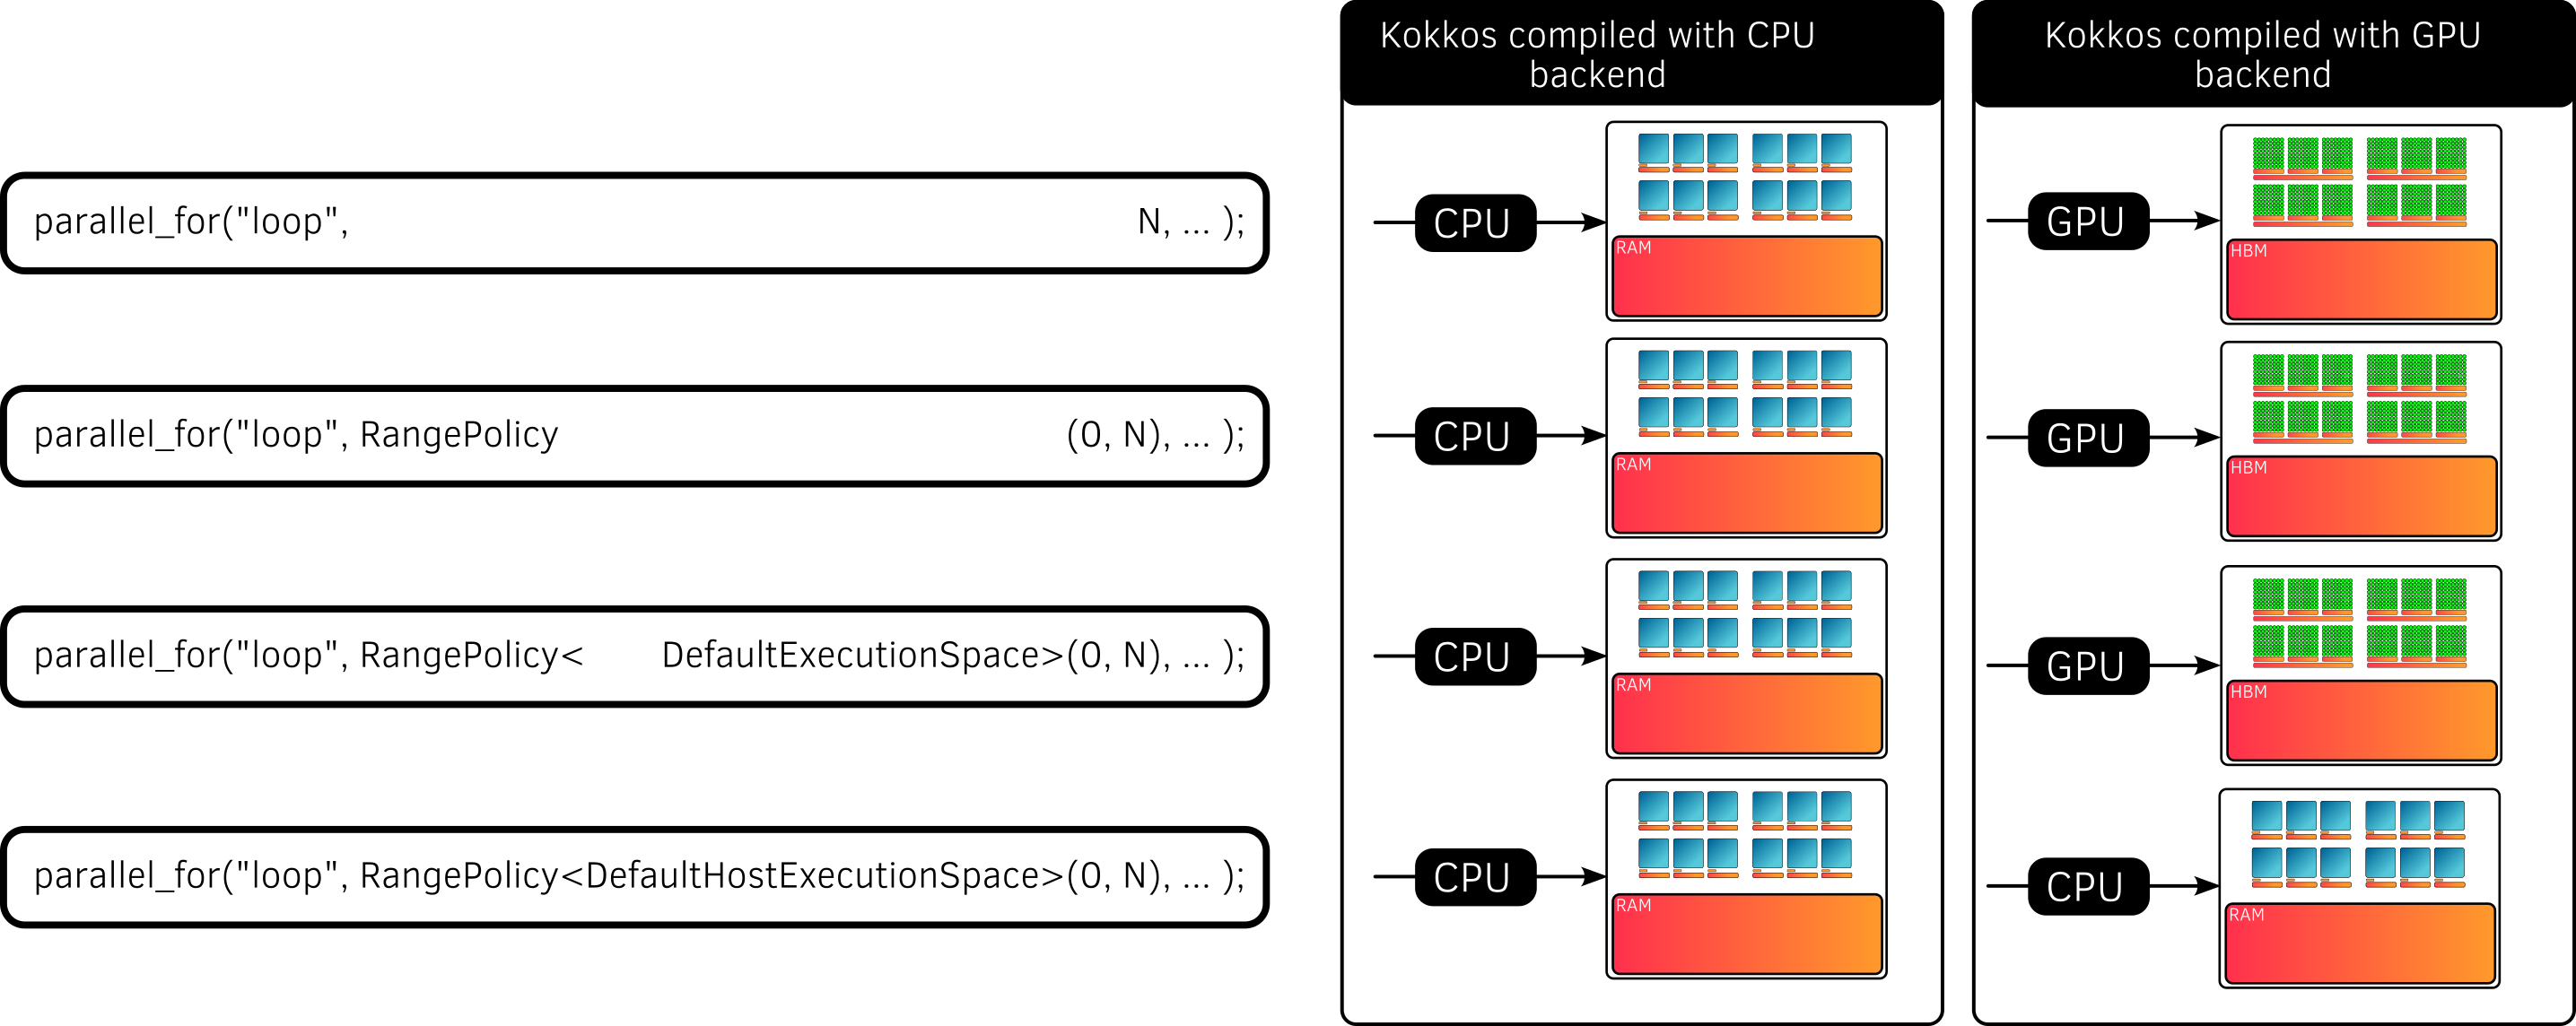
\includegraphics[width=\textwidth]{default_execution_space.png}
    \end{center}
\end{frame}

\begin{frame}[fragile]{Relation between execution space and memory space}
    \begin{itemize}
        \item That relation makes sense (both on same hardware)
        \item \texttt{memory\_space} attribute to access the memory space associated with an execution space
        \item \texttt{HostSpace} for memory space of the default host execution space
    \end{itemize}
    \pause
    \begin{center}
        \small
        \begin{table}{Default memory spaces}{lll}
            & \multicolumn{2}{l}{Kokkos compiled on} \\
            Memory space & CPU backend & GPU backend \\\hline
            \texttt{Kokkos::DefaultExecutionSpace::memory\_space} & On CPU & On GPU \\
            \texttt{Kokkos::DefaultHostExecutionSpace::memory\_space} & On CPU & On CPU
        \end{table}
    \end{center}
\end{frame}

\section{Performance}

\begin{frame}{The Ruche supercomputer}
    \begin{description}[Location]
        \item[Name] Ruche cluster
        \item[Location] IDRIS, Moulon, Île-de-France
        \item[CPU] Intel Xeon Gold 6230, 2.1 GHz, 20 cores per socket, 2 sockets per node
        \item[GPU] NVIDIA V100, 4 devices per node
        \item[GPU] NVIDIA A100, 4 devices per node
    \end{description}
\end{frame}

\begin{frame}{Performance result on Ruche}
    \begin{center}
        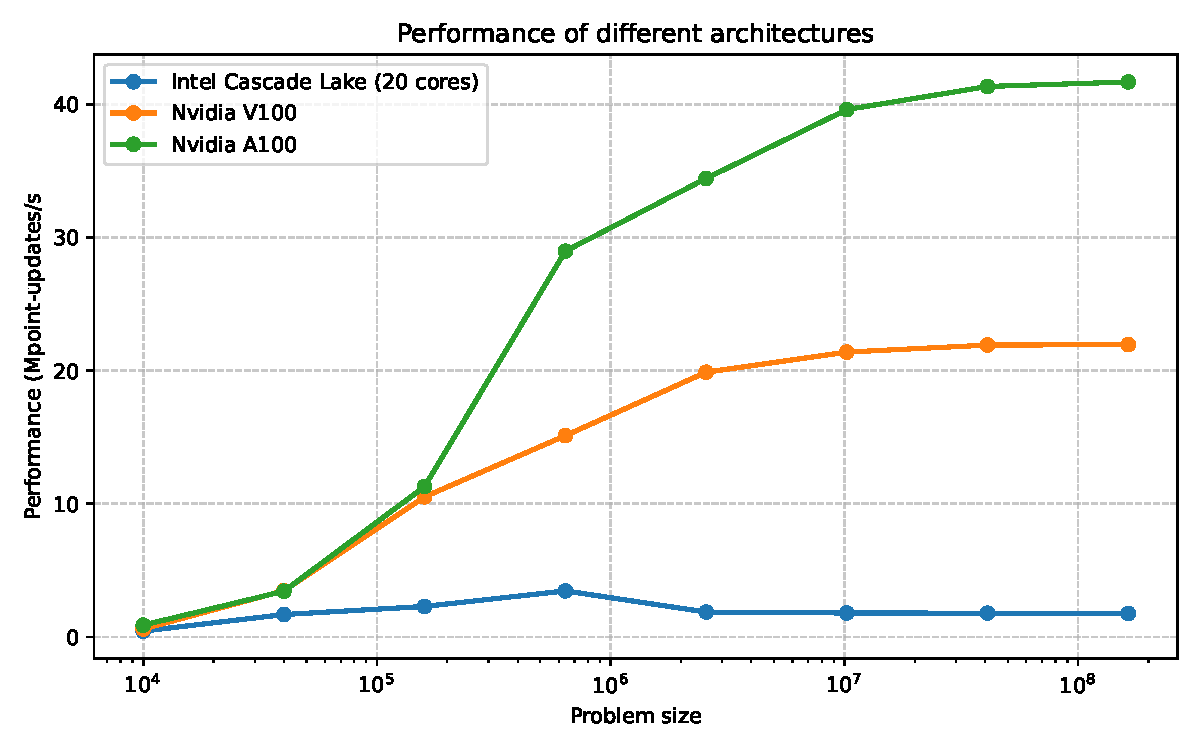
\includegraphics[width=0.8\textwidth]{performance_ruche.pdf}
    \end{center}
\end{frame}

\section{SIMD on GPU}

\begin{frame}[fragile]{What about SIMD on GPUs?}
    \begin{itemize}
        \item We said in the previous session that we cannot use vectorized CPU instructions on GPU
        \item But we just used SIMD inside a \texttt{Kokkos::parallel\_for}
        \item To keep portability, we default to a scalar type when using a GPU backend
    \end{itemize}

    \begin{center}
        \small
        \begin{table}{SIMD types}{lll}
            & \multicolumn{2}{l}{Kokkos compiled on} \\
            SIMD alias & CPU backend & GPU backend \\\hline
            \texttt{simd<T>} & \texttt{basic\_simd<T, abi<...>>} & \texttt{basic\_simd<T, scalar>} \\
            \texttt{simd<T, N>} & \texttt{basic\_simd<T, abi<N>>} & \texttt{basic\_simd<T, scalar>} \\
            \texttt{basic\_simd<T, abi<N>>} & \texttt{basic\_simd<T, abi<N>>} & \texttt{basic\_simd<T, abi<N>>}
        \end{table}
    \end{center}
\end{frame}

\begin{exerciseframe}{From the "cpu\_more\_simd" folder (optional)}
    \begin{itemize}
        \item Apply the same modifications we have done so far in the \texttt{cpu\_simd} folder
    \end{itemize}
\end{exerciseframe}

\section{Asynchronous execution}

\begin{exerciseframe}{(Re-)Initialization}
    \begin{columns}
        \begin{column}{0.65\linewidth}
            \begin{minted}[breakafter={/},fontsize=\scriptsize]{sh}
                # pick one
                IMAGE=kokkos_gpu_interactive
                IMAGE=kokkos_gpu_interactive_jupyter
                IMAGE=kokkos_gpu_interactive_vscode
                IMAGE=kokkos_gpu_learning_platform_code_server

                srun ... --pty /bin/bash

                apptainer run --nv ${IMAGE}_latest.sif

                cd $HOME/gray_scott_kokkos/exercises
            \end{minted}
        \end{column}
        \begin{column}{0.35\linewidth}
            \begin{itemize}
                \item Take the desired image:
                \begin{itemize}
                    \item No editor
                    \item Jupyter
                    \item VSCode
                    \item CodeServer
                \end{itemize}
                \item Reserve a job for the day/half a day (ask your satellite staff)
                \item Run Apptainer with the downloaded SIF image
            \end{itemize}
        \end{column}
    \end{columns}
\end{exerciseframe}

\begin{frame}{Asynchronous behavior in Kokkos}
    \begin{columns}
        \begin{column}{0.6\linewidth}
            \begin{table}{Kokkos asynchronism on GPU}{ll}
                Function & Behavior \\\hline
                \texttt{parallel\_for(/* ... */)} & Async. \\
                \texttt{parallel\_reduce(/* ... */)} & Sync. \\
                \texttt{deep\_copy(/* ... */)} & Sync. \\
                \texttt{deep\_copy(space, /* ... */)} & Async. \\
            \end{table}
        \end{column}
        \begin{column}{0.4\linewidth}
            \begin{block}{Rule of thumb}
                If a Kokkos function can take an execution space, then the version with it is asynchronous, and the version without is synchronous
            \end{block}
        \end{column}
    \end{columns}
\end{frame}

\begin{frame}{When to use asynchronism}
    \begin{itemize}
        \item As mentioned in the Fencing section, most GPU code is asynchronous by default
        \item When starting the porting to GPU, a synchronous behavior is preferred (simpler workflow, easier to debug)
        \item Asynchronous execution comes into play for optimization
        \item It is useful to hide a task that takes time by running it concurrently
        \item Need to perform a workflow analysis
    \end{itemize}
\end{frame}

\begin{frame}{What is the current workflow?}
    \begin{columns}
        \begin{column}{0.4\linewidth}
            \caption{Profiling of a 1000 by 1000 case \\ on a A500 GPU}
            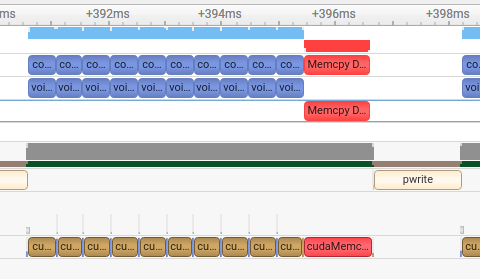
\includegraphics[width=\linewidth]{profile_gpu}

            \begin{enumerate}
                \item 10 computes \structure{(GPU)}
                \item 1 copy D-to-H \structure{(GPU-CPU)}
                \item 1 write \structure{(CPU)}, slow because of the filesystem
            \end{enumerate}
        \end{column}
        \pause
        \begin{column}{0.6\linewidth}
            \centering
            \begin{tikzpicture}[node distance=1em]
                \node (compute) {compute $\times$ 10};
                \node[below=of compute] (copy-d-to-h) {copy D-to-H};
                \node[below=of copy-d-to-h] (write) {write};

                \draw[->] (compute) -- (copy-d-to-h);
                \draw[->] (copy-d-to-h) -- (write);

                \begin{uncoverenv}<3->
                    \node[above=of compute] (write-before) {write};
                    \node[below=of write] (compute-after) {compute $\times$ 10};

                    \draw[->] (write-before) -- (compute);
                    \draw[->] (write) -- (compute-after);
                \end{uncoverenv}

                \begin{uncoverenv}<4->
                    \node[above=of write-before] (ellipsis-before) {...};
                    \node[below=of compute-after] (ellipsis-after) {...};

                    \draw[->] (ellipsis-before) -- (write-before);
                    \draw[->] (compute-after) -- (ellipsis-after);
                \end{uncoverenv}
            \end{tikzpicture}
        \end{column}
    \end{columns}
\end{frame}

\begin{frame}{Exhibit asynchronism in the workflow}
    \begin{columns}
        \begin{column}{0.5\linewidth}
            \centering
            \begin{tikzpicture}[node distance=1em]
                \node (compute) {compute $\times$ 10};
                \node[below=of compute] (copy-d-to-h) {copy-D-to-H};
                \node[below=of copy-d-to-h] (write) {write};

                \draw[->] (compute) -- (copy-d-to-h);
                \draw[->] (copy-d-to-h) -- (write);

                \node[above=of compute] (write-before) {write};
                \node[below=of write] (compute-after) {compute $\times$ 10};

                \draw[->] (write-before) -- (compute);
                \draw[->] (write) -- (compute-after);

                \node[above=of write-before] (ellipsis-before) {...};
                \node[below=of compute-after] (ellipsis-after) {...};

                \draw[->] (ellipsis-before) -- (write-before);
                \draw[->] (compute-after) -- (ellipsis-after);
            \end{tikzpicture}
        \end{column}
        \begin{column}{0.5\linewidth}
            \centering
            \begin{uncoverenv}<3->
                \begin{tikzpicture}[node distance=1em]
                    \node (compute) {compute $\times$ 10};
                    \node[below=of compute] (copy-d-to-h) {copy D-to-H};
                    \node[below=of copy-d-to-h] (write) {write};

                    \draw[->] (compute) -- (copy-d-to-h);
                    \draw[->] (copy-d-to-h) -- (write);

                    \node[left=of compute] (write-before) {write};
                    \node[right=of write] (compute-after) {compute $\times$ 10};

                    \draw[->] (copy-d-to-h) -- (compute-after);

                    \node[above=of write-before] (ellipsis-before) {...};
                    \node[below=of compute-after] (ellipsis-after) {...};

                    \draw[->] (ellipsis-before) -- (compute);
                    \draw[->] (write-before) -- (copy-d-to-h);
                    \draw[->] (ellipsis-before) -- (write-before);
                    \draw[->] (compute-after) -- (ellipsis-after);
                    \draw[->] (write) -- (ellipsis-after);
                \end{tikzpicture}
            \end{uncoverenv}
        \end{column}
    \end{columns}
    \begin{uncoverenv}<2->
        \begin{block}{Idea}
            Computation and writing can happen at the same time, as data are independent
        \end{block}
    \end{uncoverenv}
\end{frame}

\begin{exerciseframe}{From your worktree or the "gpu\_base" folder}
    \begin{columns}
        \begin{column}{0.5\linewidth}
            \centering
            \begin{tikzpicture}[node distance=1em]
                \node (compute) {compute $\times$ 10};
                \node[below=of compute] (copy-d-to-h) {copy D-to-H};
                \node[below=of copy-d-to-h] (write) {write};

                \draw[->] (compute) -- (copy-d-to-h);
                \draw[->] (copy-d-to-h) -- (write);

                \node[left=of compute] (write-before) {write};
                \node[right=of write] (compute-after) {compute $\times$ 10};

                \draw[->] (copy-d-to-h) -- (compute-after);

                \node[above=of write-before] (ellipsis-before) {...};
                \node[below=of compute-after] (ellipsis-after) {...};

                \draw[->] (ellipsis-before) -- (compute);
                \draw[->] (write-before) -- (copy-d-to-h);
                \draw[->] (ellipsis-before) -- (write-before);
                \draw[->] (compute-after) -- (ellipsis-after);
                \draw[->] (write) -- (ellipsis-after);
            \end{tikzpicture}
        \end{column}
        \begin{column}{0.5\linewidth}
            \begin{itemize}
                \item Just in the \texttt{main} function
                \item Re-consider the loop
                \begin{itemize}
                    \item One loop for the images
                    \item One loop for the iterations per image
                \end{itemize}
                \item Roll the operations of the loop
                \item Take care of the boundary effects
                \item Adjust the fences
                \pause
                \item Beware, there is a subtlety on CPU
                \item Make it run correctly on CPU
            \end{itemize}
        \end{column}
    \end{columns}
\end{exerciseframe}

\begin{frame}[fragile]{Kokkos asynchronism within the GPU}
    \begin{columns}
        \begin{column}{0.4\linewidth}
            \begin{itemize}
                \item We saw how to hide a CPU task by running it concurrently with a GPU task
                \item GPU has streams/queues that allow multiples kernels to run concurrently
                \item Kokkos has the \texttt{partition\_space} function for this
                \item Returns a vector of execution space instances
                \item Weights only used by the OpenMP backend for now
            \end{itemize}
        \end{column}
        \begin{column}{0.6\linewidth}
            \begin{minted}[breakafter={:}]{C++}
                auto instances = Kokkos::Experimental::partition_space(
                    Kokkos::DefaultExecutionSpace {},
                    weight_1,
                    weight_2,
                    /* ... */
                );

                Kokkos::parallel_for(
                    "my streamed kernel",
                    Kokkos::RangePolicy(
                        instances[0], 0, N
                    ),
                    /* ... */
                );
            \end{minted}
        \end{column}
    \end{columns}
\end{frame}

\begin{frame}{What is the current workflow?}
        \begin{columns}
        \begin{column}{0.4\linewidth}
            \caption{Profiling of a 1000 by 1000 case \\ on a A500 GPU}

            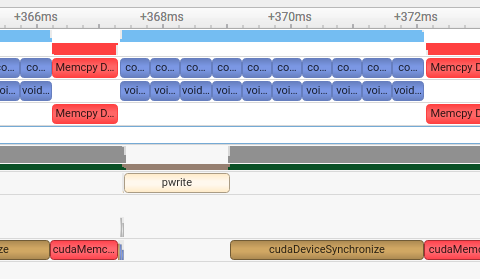
\includegraphics[width=\linewidth]{profile_gpu_async}

            \begin{enumerate}
                \item 1 copy D-to-H \structure{(GPU-CPU)}, slow because of the PCIe bus
                \item 10 computations \structure{(GPU)}
                \item 1 write \structure{(CPU, hidden)}
            \end{enumerate}
        \end{column}
        \pause
        \begin{column}{0.6\linewidth}
            \centering
            \begin{tikzpicture}[node distance=1em]
                \node (compute) {compute $\times$ 10};
                \node[below=of compute] (copy-d-to-h) {copy D-to-H};
                \node[below=of copy-d-to-h] (write) {write};

                \draw[->] (compute) -- (copy-d-to-h);
                \draw[->] (copy-d-to-h) -- (write);

                \node[left=of compute] (write-before) {write};
                \node[right=of write] (compute-after) {compute $\times$ 10};

                \draw[->] (copy-d-to-h) -- (compute-after);

                \node[above=of write-before] (ellipsis-before) {...};
                \node[below=of compute-after] (ellipsis-after) {...};

                \draw[->] (ellipsis-before) -- (compute);
                \draw[->] (write-before) -- (copy-d-to-h);
                \draw[->] (ellipsis-before) -- (write-before);
                \draw[->] (compute-after) -- (ellipsis-after);
                \draw[->] (write) -- (ellipsis-after);
            \end{tikzpicture}
        \end{column}
    \end{columns}
\end{frame}

\begin{frame}{Exhibit more asynchronism in the workflow}
    \begin{columns}
        \begin{column}{0.4\linewidth}
            \centering
            \begin{tikzpicture}[node distance=1em]
                \node (compute) {compute $\times$ 10};
                \node[below=of compute] (copy-d-to-h) {copy D-to-H};
                \node[below=of copy-d-to-h] (write) {write};

                \draw[->] (compute) -- (copy-d-to-h);
                \draw[->] (copy-d-to-h) -- (write);

                \node[left=of compute] (write-before) {write};
                \node[right=of write] (compute-after) {compute $\times$ 10};

                \draw[->] (copy-d-to-h) -- (compute-after);

                \node[above=of write-before] (ellipsis-before) {...};
                \node[below=of compute-after] (ellipsis-after) {...};

                \draw[->] (ellipsis-before) -- (compute);
                \draw[->] (write-before) -- (copy-d-to-h);
                \draw[->] (ellipsis-before) -- (write-before);
                \draw[->] (compute-after) -- (ellipsis-after);
                \draw[->] (write) -- (ellipsis-after);
            \end{tikzpicture}
        \end{column}
        \begin{column}{0.6\linewidth}
            \centering
            \begin{uncoverenv}<3->
                \begin{tikzpicture}[node distance=1em]
                    \node (compute) {compute $\times$ 10};
                    \node[below=3em of compute] (copy-d-to-d) {copy D-to-D};
                    \node[below=of copy-d-to-d] (copy-d-to-h) {copy D-to-H};
                    \node[below=of copy-d-to-h] (write) {write};

                    \draw[->] (compute) -- (copy-d-to-d);
                    \draw[->] (copy-d-to-d) -- (copy-d-to-h);
                    \draw[->] (copy-d-to-h) -- (write);

                    \node[left=of compute] (copy-d-to-h-before) {copy D-to-H};
                    \node[below=of copy-d-to-h-before] (write-before) {write};
                    \node[right=of copy-d-to-h] (compute-after) {compute $\times$ 10};

                    \draw[->] (copy-d-to-d) -- (compute-after);

                    \node[above=of copy-d-to-h-before] (ellipsis-before) {...};
                    \node[below=3em of compute-after] (ellipsis-after) {...};

                    \draw[->] (ellipsis-before) -- (compute);
                    \draw[->] (write-before) -- (copy-d-to-d);
                    \draw[->] (ellipsis-before) -- (copy-d-to-h-before);
                    \draw[->] (copy-d-to-h-before) -- (write-before);
                    \draw[->] (compute-after) -- (ellipsis-after);
                    \draw[->] (write) -- (ellipsis-after);
                \end{tikzpicture}
            \end{uncoverenv}
        \end{column}
    \end{columns}
    \begin{uncoverenv}<2->
        \begin{block}{Idea}
            Copy D-to-H can be viewed as copy D-to-D, then copy D-to-H
        \end{block}
    \end{uncoverenv}
\end{frame}

\begin{exerciseframe}{\small From your worktree or the "gpu\_more\_async\_0\_write" folder}
    \begin{columns}
        \begin{column}{0.6\linewidth}
            \centering
            \begin{tikzpicture}[node distance=1em]
                \node (compute) {compute $\times$ 10};
                \node[below=3em of compute] (copy-d-to-d) {copy D-to-D};
                \node[below=of copy-d-to-d] (copy-d-to-h) {copy D-to-H};
                \node[below=of copy-d-to-h] (write) {write};

                \draw[->] (compute) -- (copy-d-to-d);
                \draw[->] (copy-d-to-d) -- (copy-d-to-h);
                \draw[->] (copy-d-to-h) -- (write);

                \node[left=of compute] (copy-d-to-h-before) {copy D-to-H};
                \node[below=of copy-d-to-h-before] (write-before) {write};
                \node[right=of copy-d-to-h] (compute-after) {compute $\times$ 10};

                \draw[->] (copy-d-to-d) -- (compute-after);

                \node[above=of copy-d-to-h-before] (ellipsis-before) {...};
                \node[below=3em of compute-after] (ellipsis-after) {...};

                \draw[->] (ellipsis-before) -- (compute);
                \draw[->] (write-before) -- (copy-d-to-d);
                \draw[->] (ellipsis-before) -- (copy-d-to-h-before);
                \draw[->] (copy-d-to-h-before) -- (write-before);
                \draw[->] (compute-after) -- (ellipsis-after);
                \draw[->] (write) -- (ellipsis-after);
            \end{tikzpicture}
        \end{column}
        \begin{column}{0.4\linewidth}
            \begin{itemize}
                \item Create the duplicated view
                \item Create one stream for computation, and one for duplication, with \texttt{partition\_space}
                \begin{itemize}
                    \item One stream for \texttt{parallel\_for}
                    \item One stream for \texttt{deep\_copy}
                \end{itemize}
                \item Differentiate the \texttt{deep\_copy} for the duplication and for the synchronization
                \item Adjust the fences
                \pause
                \item Beware, there is a subtlety on CPU
                \item Make it run correctly on CPU
            \end{itemize}
        \end{column}
    \end{columns}
\end{exerciseframe}

\begin{frame}{A word about graphs}
    \begin{itemize}
        \item The \emph{workflow} we analyzed before can also be called a graph
        \item CUDA/HIP has a task-based graph approach
        \item SYCL has a data-based graph approach
        \pause
        \item Kokkos provides a graph API (very similar with the CUDA graph API)
        \item It expresses the workflow clearly, without having to manage the execution spaces manually
        \pause
        \item Still experimental and not complete enough for our example
    \end{itemize}
\end{frame}

\section{Atomics}

\begin{frame}[fragile]{Race condition}
    Porting a code creating a histogram:
    \begin{columns}
        \begin{column}{0.5\linewidth}
            \begin{minted}{C++}
                double histo[5] = {0};

                for (int i=0; i < N; i++) {
                    histo[i % 5] += i;
                }
            \end{minted}
        \end{column}
        \pause
        \begin{column}{0.5\linewidth}
            \begin{minted}{C++}
                Kokkos::View<double*> histo(5);

                Kokkos::parallel_for(
                N,
                KOKKOS_LAMBDA(int i) {
                    histo(i % 5) += i;
                });
            \end{minted}
        \end{column}
    \end{columns}
\end{frame}

\colorlet{lightmain2}{lightmain!50}

\begin{frame}[fragile]{Race condition}
    \begin{columns}
        \begin{column}{0.55\linewidth}
            Even simple instructions like increment are decomposed into several smaller assembly instructions:
            \begin{minted}{C++}
                histo(i % 5) += i;
            \end{minted}
        \end{column}
        \begin{column}{0.45\linewidth}
            \small
            \begin{table}{Operations}{llcl}
                \textbf{Thread 1} & \textbf{Thread 6} &  & \textbf{Result} \\\hline
                & & & 0 \\
                \rowcolor{lightmain}read value & & $\leftarrow$ & 0 \\
                \rowcolor{lightmain}add 1 & &  & 0 \\
                \rowcolor{lightmain}write value & & $\rightarrow$ & 1 \\
                & & & 1 \\
                \rowcolor{lightmain2}& read value & $\leftarrow$ & 1 \\
                \rowcolor{lightmain2}& add 6 &  & 1 \\
                \rowcolor{lightmain2}& write value & $\rightarrow$ & 7 \\
                & & & 7 \\
            \end{table}
        \end{column}
    \end{columns}
\end{frame}

\begin{frame}[fragile]{Race condition}
    \begin{columns}
        \begin{column}{0.55\linewidth}
            Execution between threads is independent. There is no guarantee over the order of instructions:
            \begin{minted}{C++}
                histo(i % 5) += i;
            \end{minted}

            When several threads are accessing the same data, it will generate \structure{race conditions}.
        \end{column}
        \begin{column}{0.45\linewidth}\\
            \small
            \begin{table}{Operations}{llcl}
                \textbf{Thread 1} & \textbf{Thread 6} &  & \textbf{Result} \\\hline
                & & & 0 \\
                \rowcolor{lightmain}read value & & $\leftarrow$ & 0 \\
                \rowcolor{lightmain2}& read value & $\leftarrow$ & 0 \\
                \rowcolor{lightmain}add 1 & & & 0 \\
                \rowcolor{lightmain}write value & & $\rightarrow$ & 1 \\
                & & & 1 \\
                \rowcolor{lightmain2}& add 6 & & 1 \\
                \rowcolor{lightmain2}& write value & $\rightarrow$ & 6 \\
                & & & 6 \\
            \end{table}
        \end{column}
    \end{columns}
\end{frame}

\begin{frame}[fragile]{Atomic operation}
    Replacing the addition with its atomic counterpart solves the problem:
    \begin{columns}
        \begin{column}{0.40\linewidth}
            \begin{minted}{C++}
                Kokkos::parallel_for(
                    N,
                    KOKKOS_LAMBDA(int i) {
                        histo(i % 5) += i;
                    }
                );
            \end{minted}
        \end{column}
        \begin{column}{0.56\linewidth}
            \begin{minted}{C++}
                Kokkos::parallel_for(
                    N,
                    KOKKOS_LAMBDA(int i) {
                        Kokkos::atomic_add(&histo(i % 5), i);
                    }
                );
            \end{minted}
        \end{column}
    \end{columns}
    \structure{Note:} \texttt{atomic\_add} takes a pointer and not a
    reference as first argument, as the instruction needs to have an access to
    the actual memory address of the modified variable.
\end{frame}

\begin{frame}[fragile]{Atomic operation}
    \begin{columns}
        \begin{column}{0.55\linewidth}
            \texttt{atomic\_add} executes the write, read and add in a single atomic step,
            guarantying the absence of race conditions during the operation:
            \begin{minted}{C++}
                Kokkos::atomic_add(&histo(i % 5), i);
            \end{minted}
        \end{column}
        \begin{column}{0.45\linewidth}
            \vspace{-0.5em}

            \small
            \begin{table}{Operations}{llcl}
                \textbf{Thread 1} & \textbf{Thread 6} &  & \textbf{Result} \\\hline
                & & & 0 \\
                \rowcolor{lightmain}atomic add & & $\leftrightarrow$ & 1 \\
                \rowcolor{lightmain2}& atomic add & $\leftrightarrow$ & 7 \\
                &  &  & 7 \\
            \end{table}
            \pause
            \begin{table}{Operations}{llcl}
                \textbf{Thread 1} & \textbf{Thread 6} &  & \textbf{Result} \\\hline
                & & & 0 \\
                \rowcolor{lightmain}& atomic add & $\leftrightarrow$ & 6 \\
                \rowcolor{lightmain2}atomic add & & $\leftrightarrow$ & 7 \\
                &  &  & 7 \\
            \end{table}
        \end{column}
    \end{columns}
\end{frame}

\begin{frame}[fragile]{Operations}
    \begin{columns}
        \begin{column}{0.35\linewidth}
            Other common operations are available with the format \texttt{Kokkos::atomic\_[op]}:
        \end{column}
        \begin{column}{0.75\linewidth}
            \footnotesize
            \begin{table}{Atomic operators}{ll}
                Operation & Replaces \\\hline
                \texttt{Kokkos::atomic\_add(\&x, y)}    & \texttt{x += y} \\
                \texttt{Kokkos::atomic\_sub(\&x, y)}    & \texttt{x -= y} \\
                \texttt{Kokkos::atomic\_mul(\&x, y)}    & \texttt{x *= y} \\
                \texttt{Kokkos::atomic\_div(\&x, y)}    & \texttt{x /= y} \\
                \texttt{Kokkos::atomic\_and(\&x, y)}    & \texttt{x \&= y} \\
                \texttt{Kokkos::atomic\_or(\&x, y)}     & \texttt{x |= y} \\
                \texttt{Kokkos::atomic\_xor(\&x, y)}    & \texttt{x \^{}= y} \\
                \texttt{Kokkos::atomic\_max(\&x, y)}    & \texttt{x = std::max(x, y)} \\
                \texttt{Kokkos::atomic\_min(\&x, y)}    & \texttt{x = std::min(x, y)} \\
                \texttt{Kokkos::atomic\_store(\&x, y)}  & \texttt{x = y} \\
                ... & ... \\
            \end{table}
        \end{column}
    \end{columns}
\end{frame}

\begin{frame}[fragile]{Atomic Memory Trait}
    \begin{columns}
        \begin{column}{0.40\linewidth}
            \begin{itemize}
                \item If you need to access a View exclusively through atomic operations, you
                can also create an alias with the \texttt{Atomic} memory trait
                \item It guarantees that any operation done through the alias are done atomically
            \end{itemize}
        \end{column}
        \begin{column}{0.6\linewidth}
            \vspace{-0.5em}

            \begin{minted}{C++}
                Kokkos::View<double*> histo(5);

                Kokkos::View<
                    double*,
                    Kokkos::MemoryTraits<Kokkos::Atomic>
                > histo_atomic = histo;

                Kokkos::parallel_for(
                    N,
                    KOKKOS_LAMBDA(int i) {
                        histo_atomic(i % 5) += i;
                    }
                );
            \end{minted}
        \end{column}
    \end{columns}
    \structure{Note:} It is preferable to give an explicit name to the alias because it will be the only way to know that the operations performed on it are atomics.
\end{frame}

\begin{frame}[fragile]{Performances}
    \begin{columns}
        \begin{column}{0.45\linewidth}
            Atomics can have a huge impact on performance:
            \begin{itemize}
                \item The instruction itself is slower than the one it replaces
                \item They may generate extra synchronisation points
                \item They bypass and invalidate cache lines
            \end{itemize}
        \end{column}
        \begin{column}{0.55\linewidth}
            \begin{block}{Remarks}
                \begin{itemize}
                    \item Atomics should be used with care and only when strictly
                    necessary
                    \item Algorithm can sometime be changed when porting from CPU to GPU
                    in order to remove the need for atomics (coloring, replacing in
                    place algorithm with out of place algorithm, etc.)
                \end{itemize}
            \end{block}
        \end{column}
    \end{columns}
\end{frame}

\section{Algorithms API}

\begin{frame}[fragile]{Acknowledgment}
    Francesco Rizzi, \emph{Implementing the C++ std algorithms library in
    Kokkos: an overview of the main challenges, API differences and
    some implementation details}, Café Kokkos @ CEA, Feb. 2024.
\end{frame}

\begin{frame}[fragile]{Inspired by STL Algorithms in C++}
    \begin{itemize}
        \item Free functions that operate on a range of elements:
        sorting, searching, counting, transforming etc
        \item Goal: Ready to use and reliable
        \begin{itemize}
            \item Internally use \texttt{Kokkos::parallel\_\{for, reduce, scan\}}
        \end{itemize}
        \item Higher abstraction in user code: Function call with a range of elements, operations etc
        \item Mostly in \texttt{Kokkos::Experimental} namespace
        \begin{itemize}
            \item Except for Sort
            \item Also, there is Random in \texttt{Kokkos} namespace
        \end{itemize}
    \end{itemize}

\end{frame}

\begin{frame}[fragile]{Currently available functions}
    \vspace{-0.5em}

    \small
    \begin{table}{Functions}{ll}
        Algorithm family & Functions \\\hline
        Sorting and related & \texttt{sort}, \texttt{sort\_by\_key}, \texttt{is\_sorted}, \texttt{is\_sorted\_until} \\
        Minimum/maximum  & \texttt{min\_element}, \texttt{max\_element}, \texttt{minmax\_element} \\
        Modifying sequence  & \makecell[l]{\texttt{copy}, \texttt{move}, \texttt{fill}, \texttt{transform}, \texttt{remove}, \texttt{replace}, \texttt{reverse}, \\\texttt{rotate}, \texttt{unique}, ...} \\
        Non-modifying sequence & \texttt{count}, \texttt{equal}, \texttt{all\_of}, \texttt{any\_of}, \texttt{find}, \texttt{for\_each}, \texttt{search}, ... \\
        Numeric & \makecell[l]{\texttt{adjacent\_difference}, \texttt{reduce}, \texttt{exclusive\_scan}, \\\texttt{inclusive\_scan}, ...} \\
        Partitioning & \texttt{is\_partitioned}, \texttt{partition\_point}, \texttt{partition\_copy} \\
        Iterators & \texttt{begin}, \texttt{cbegin}, \texttt{end}, \texttt{cend}, \texttt{distance}, \texttt{iter\_swap} \\
        Random & \texttt{Random\_XorShift64\_Pool}, ...
    \end{table}

    \vspace{0.5em}

    More in the \href{https://kokkos.org/kokkos-core-wiki/API/algorithms-index.html}{documentation}
\end{frame}

\begin{frame}[fragile]{API usage}
    Pass to the function:
    \begin{itemize}
        \item Execution space instance
        \begin{itemize}
            \item Team Handle under Hierarchical parallelism also possible
            \item Not elegant. For now, needed by algorithms in \texttt{Kokkos::Experimental} namespace
            \item Deducing execution space from Views or Iterators is the better way
        \end{itemize}
        \item A Rank-1 View or begin and end Iterators
        \begin{itemize}
            \item View must be accessible from the execution space
            \item The Iterators are random access, obtained via \texttt{Kokkos::Experimental::\{begin, cbegin, end, cend\}}
        \end{itemize}
        \item Additional function specific arguments
    \end{itemize}
    \begin{minted}{C++}
        auto ret_val_view = algo_name(label, space, view(s), extra_args);
        auto ret_val_iterator =
            algo_name(label, space, iterator(s), extra_args);
    \end{minted}
\end{frame}

\begin{frame}[fragile]{Example usage}
    \begin{minted}{C++}
        namespace KE = Kokkos::Experimental;

        Kokkos::View<double*> my_view("my_view", 13);
        // In general, View must be accessible from execution space
        // Fill my_view

        const double old_val{2}, new_val{34};
        auto def_exec_space = Kokkos::DefaultExecutionSpace();

        // act on the entire view
        KE::replace(def_exec_space, my_view, old_val, new_val);

        // act on just a subset
        auto start_at = KE::begin(my_view) + 4;
        auto end_at = KE::begin(my_view) + 10;
        KE::replace(def_exec_space, start_at, end_at, old_val, new_val);
    \end{minted}
\end{frame}

\begin{frame}[fragile]{Example usage}
    \begin{minted}{C++}
        struct MyStruct { /* ... */ }; // Custom type

        struct MyStructLessThanComparator {
            bool operator()(const MyStruct& a, const MyStruct& b) const {
                // custom comparator logic
            }
        };

        int main() {
            Kokkos::View<MyStruct*> my_view("my_view", N);
            // ...
            KE::min_element(
                def_exec_space, my_view, MyStructLessThanComparator());
            // ...
        }
    \end{minted}
\end{frame}

\section{Kokkos ecosystem}

\begin{frame}{Kokkos ekosystem}
    \begin{center}
        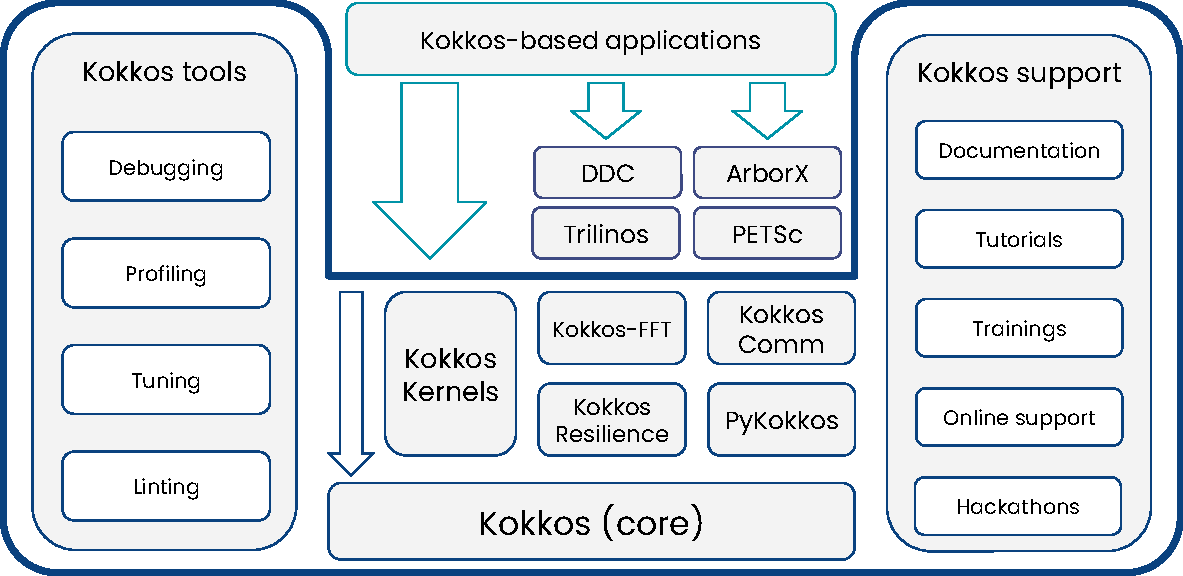
\includegraphics[width=0.9\textwidth]{ekokkosystem}
    \end{center}
\end{frame}

\begin{frame}{Kokkos-FFT}
    \begin{columns}
        \begin{column}{0.5\linewidth}
            \begin{itemize}
                \item What is it?
                \begin{itemize}
                    \item Fast Fourier Transform (FFT) interface integrated into the Kokkos ecosystem
                    \item Enables portable FFT computations on heterogeneous systems
                \end{itemize}
                \item Why it matters?
                \begin{itemize}
                    \item FFT libraries are usually hardware-specific
                    \item Managing CPU/GPU differences is complex
                \end{itemize}
            \end{itemize}
        \end{column}
        \begin{column}{0.5\linewidth}
            \begin{itemize}
                \item Key features
                \begin{itemize}
                    \item Supports 1D, 2D, and 3D FFTs
                    \item Works directly with Kokkos Views
                    \item Backend abstraction (e.g., FFTW, cuFFT)
                \end{itemize}
            \end{itemize}
        \end{column}
    \end{columns}
\end{frame}

\begin{frame}[fragile]{2D FFT example}
    \begin{minted}[fontsize=\small]{C++}
        const Kokkos::complex<double> z(1.0, 1.0);

        // 2D C2C FFT (Forward and Backward)
        const Kokkos::View<Kokkos::complex<double>**>
            xc2c("xc2c", n0, n1),
            xc2c_hat("xc2c_hat", n0, n1),
            xc2c_inv("xc2c_inv", n0, n1);

        Kokkos::Random_XorShift64_Pool<> random_pool(12345);
        Kokkos::DefaultExecutionSpace exec_space;
        Kokkos::fill_random(exec_space, xc2c, random_pool, z);

        KokkosFFT::fft2(exec_space, xc2c, xc2c_hat);
        KokkosFFT::ifft2(exec_space, xc2c_hat, xc2c_inv);
    \end{minted}
\end{frame}

\begin{frame}{Kokkos Kernels}
    \begin{columns}
        \begin{column}{0.5\linewidth}
            \begin{itemize}
                \item What is it?
                \begin{itemize}
                    \item Library of optimized parallel kernels built on Kokkos
                    \item Provides standard HPC building blocks (BLAS, sparse, graph)
                \end{itemize}
                \item Why it matters?
                \begin{itemize}
                    \item Avoid reimplementing performance-critical kernels
                    \item Tuned for CPUs, GPUs, and manycore systems
                    \item Ensures portability without sacrificing performance
                \end{itemize}
            \end{itemize}
        \end{column}
        \begin{column}{0.5\linewidth}
            \begin{itemize}
                \item Key features
                \begin{itemize}
                    \item Dense linear algebra (BLAS-level operations)
                    \item Sparse matrix operations (SpMV, SpGEMM, triangular solves)
                    \item Graph kernels and utilities
                \end{itemize}
            \end{itemize}
        \end{column}
    \end{columns}
\end{frame}

\begin{frame}[fragile]{GEMV example}
    \begin{minted}[fontsize=\scriptsize]{C++}
        Kokkos::View<double**> A("A", n, m);
        Kokkos::View<double*> x("x", m), y("y", n);

        Kokkos::parallel_for("InitA", N, KOKKOS_LAMBDA(int i) {
            for (int j = 0; j < m; j++) {
                A(i,j) = i + j + 1.0;
            }
        });

        Kokkos::parallel_for("InitX", m, KOKKOS_LAMBDA(int i) { x(i) = 1.0; });
        Kokkos::parallel_for("InitY", n, KOKKOS_LAMBDA(int i) { y(i) = 0.0; });

        double alpha = 1.0, beta  = 0.0;
        KokkosBlas::gemv("N", alpha, A, x, beta, y);

        // check outcome
        auto y_host = Kokkos::create_mirror_view_and_copy(Kokkos::HostSpace(), y);
        for (int i = 0; i < n; i++) {
            std::cout << "y(" << i << ") = " << y_host(i) << std::endl;
        }
    \end{minted}
\end{frame}

\begin{frame}{Kokkos Comm}
    \begin{columns}
        \begin{column}{0.5\linewidth}
            \begin{itemize}
                \item What is it?
                \begin{itemize}
                    \item A lightweight C++ library for distributed communication on Kokkos
                    \item Designed for performance portability across heterogeneous systems (CPU, GPU, multi-node)
                \end{itemize}
                \item Why it matters?
                \begin{itemize}
                    \item Kokkos handles intra-node parallelism, but inter-node communication is still complex
                    \item Traditional MPI usage with Kokkos leads to:
                    \item Code duplication
                    \item Manual data packing/unpacking
                    \item Difficult GPU-aware communication
                \end{itemize}
            \end{itemize}
        \end{column}
        \begin{column}{0.5\linewidth}
            \begin{itemize}
                \item Key features
                \begin{itemize}
                    \item Performance-portable communication API
                    \item Asynchronous operations (non-blocking send/recv, collectives)
                    \item Automatic handling of:
                    \item GPU-aware communication
                    \item Non-contiguous data (Kokkos Views)
                    \item Minimal, composable, modern C++20 interface
                    \item Built on top of existing 	communication libraries:
                    \item MPI, NCCL (others under exploration)
                \end{itemize}
            \end{itemize}
        \end{column}
    \end{columns}
\end{frame}

\begin{frame}[fragile]{Distributed GEMV example}
    \vspace{-1em}

    \begin{columns}
        \begin{column}{0.8\linewidth}
            \begin{minted}[fontsize=\tiny]{C++}
                KokkosComm::Handle handle(exec_space, comm_object);

                Kokkos::View<double**> A("A", local_m, global_n); // 1D row-wise partitioning
                Kokkos::View<double*> x("x", global_n);
                Kokkos::View<double*> y("y", local_m);

                // Initialize local part of vector x on each process
                Kokkos::parallel_for(
                    "init local x",
                    Kokkos::RangePolicy(exec_space, handle.rank() * local_m, (handle.rank() + 1) * local_m),
                    KOKKOS_LAMBDA(int i) { x(i) = static_cast<double>(handle.rank * i); }
                );
                exec_space.fence();

                auto allgather_req = KokkosComm::allgather(handle, x, x);

                // Initialize local part of A on each process
                Kokkos::parallel_for(
                    "init local A",
                    Kokkos::MDRangePolicy({0, 0}, {local_m, global_n}),
                    KOKKOS_LAMBDA(int i, int j) { A(i, j) = static_cast<double>(handle.rank() + j); }
                );
                exec_space.fence();

                KokkosComm::wait(allgather_req);

                KokkosBlas::gemv("N", alpha, A, x, beta, y);
            \end{minted}
        \end{column}
        \begin{column}{0.2\linewidth}
            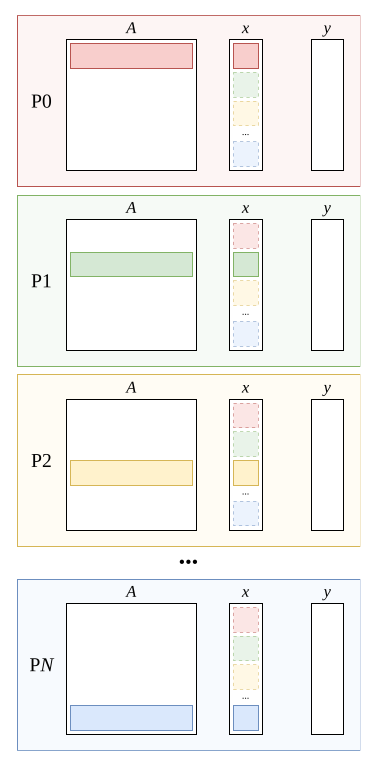
\includegraphics[width=\linewidth]{kokkos_comm_gemv}
        \end{column}
    \end{columns}
\end{frame}

\begin{frame}{Kokkos-Fortran Interop}
    \begin{columns}
        \begin{column}{0.5\linewidth}
            \begin{itemize}
                \item What is it?
                \begin{itemize}
                    \item Interoperability library
                    \item Allows Fortran programs to use Kokkos data structures and call Kokkos C++ parallel constructs
                \end{itemize}
                \item Why it matters?
                \begin{itemize}
                    \item There are large Fortran HPC codes (1 M+ lines of code)
                    \item Rewriting mature Fortran applications in C++ is costly and risky
                    \item Local impact on the code
                \end{itemize}
            \end{itemize}
        \end{column}
        \begin{column}{0.5\linewidth}
            \begin{itemize}
                \item Key features
                \begin{itemize}
                    \item Enable portable GPU acceleration for Fortran programs
                    \item Interoperability via \texttt{ISO\_C\_BINDING} module
                    \item Fortran derived-types to handle Kokkos Views, accessible with Fortran pointer arrays
                    \item SharedSpace memory for data synchronization
                \end{itemize}
            \end{itemize}
        \end{column}
    \end{columns}
\end{frame}

\begin{frame}{PyKokkos}
    \begin{columns}
        \begin{column}{0.5\linewidth}
            \begin{itemize}
                \item What is it?
                \begin{itemize}
                    \item Interoperability library
                    \item Translation layer
                \end{itemize}
                \item Why it matters?
                \begin{itemize}
                    \item Python is a popular and good prototyping language
                    \item Lowers the barrier to using Kokkos
                    \item Improves productivity for scientists and data analysts working in Python
                \end{itemize}
            \end{itemize}
        \end{column}
        \begin{column}{0.5\linewidth}
            \begin{itemize}
                \item Key features
                \begin{itemize}
                    \item Enable portable GPU acceleration for Python programs
                    \item Interoperability with Numpy and Cupy
                    \item Use main Kokkos concepts directly in Python
                    \item JIT compilation of Python code for CPU and GPU
                \end{itemize}
            \end{itemize}
        \end{column}
    \end{columns}
\end{frame}

\section{Conclusion}

\begin{frame}{Conclusion}
    \begin{itemize}
        \item Portability for GPU-only annotations
        \item Concept of memory spaces and execution spaces
        \item Fencing to force synchronous execution
        \item Kokkos-Tools
        \item Explicit memory management with mirrors
        \item GPU optimization with asynchronous execution
        \item Atomic operations
        \item Algorithms API
        \item Kokkos ecosystem
    \end{itemize}
    \pause
    \begin{block}{Congratulations}
        You can now write Kokkos portable code!
    \end{block}
\end{frame}

\begin{frame}[plain]
    \closingpage
\end{frame}

\end{document}
